% !TeX program = pdflatex
\documentclass{iutbscthesis}

\addbibresource{citations.bib}

\usepackage{amsmath}
\usepackage{enumitem}
\usepackage{booktabs}
\usepackage{graphicx}
\emergencystretch=3em

% Complete thesis title. Kept aligned with the approved IUT thesis title.
\title{Beyond Naive Parameter Sharing : A Disentangled-Head MARL Architecture for Bandwidth Constrained Vehicular OTA Updates}

\addauthor{Mahmudul Islam Mahin}{210042140}
\addauthor{Saadman Sakib}{210042165}
\addauthor{Mohtasim Dipto}{210042175}


\supervisor{Dr.\ Kamrul Hasan}{Professor}{Department of Computer Science and Engineering}
\department{Department of Computer Science and Engineering}
\program{BACHELOR OF SCIENCE IN COMPUTER SCIENCE AND ENGINEERING}
\defensedate{17}{September}{2026}

\begin{document}

%-------------------------- FRONT MATTER --------------------------%
\coverpage
\pagenumbering{roman}
\titlepage
\declarationofcandidate
\dedicatedto{our families}

\tableofcontents
\listoffigures
\listoftables
\clearpage

\begin{abbreviations}
    \abbr{ECU}{Electronic Control Unit}
    \abbr{OTA}{Over-the-Air}
    \abbr{CAV}{Connected and Autonomous Vehicle}
    \abbr{SDV}{Software-Defined Vehicle}
    \abbr{RL}{Reinforcement Learning}
    \abbr{MARL}{Multi-Agent Reinforcement Learning}
    \abbr{MDP}{Markov Decision Process}
    \abbr{Dec-POMDP}{Decentralized Partially Observable Markov Decision Process}
    \abbr{PPO}{Proximal Policy Optimization}
    \abbr{IPPO}{Independent Proximal Policy Optimization}
    \abbr{MAPPO}{Multi-Agent Proximal Policy Optimization}
    \abbr{FP3O}{Full-Pipeline Proximal Policy Optimization}
    \abbr{CTDE}{Centralized Training, Decentralized Execution}
    \abbr{CBF}{Control Barrier Function}
    \abbr{UDS}{Unified Diagnostic Services}
    \abbr{MB}{Modify+Backup / Multi-Base update operation}
    \abbr{KL}{Kullback--Leibler divergence}
    \abbr{MLP}{Multi-Layer Perceptron}
    \abbr{CI}{Confidence Interval}
\end{abbreviations}

\begin{acknowledgement}
We would like to express our sincere gratitude to our supervisor, Dr.\ Kamrul Hasan, for his guidance, critical feedback, and encouragement throughout this work. In particular, his insistence on checking apparently convenient experimental results helped us identify the observation-design confound that materially changed the interpretation of our parameter-sharing comparison.

We are grateful to the Department of Computer Science and Engineering and the Islamic University of Technology for providing the academic environment and computational resources required for this research.

Finally, we thank our families and friends for their continuous support throughout the development, debugging, experimentation, and writing of this thesis.
\end{acknowledgement}

\begin{abstract}
Automotive Over-the-Air (OTA) firmware updating is a constrained scheduling problem in which heterogeneous Electronic Control Units (ECUs) must be updated without exceeding device-memory limits while sharing a communication gateway whose available bandwidth may fluctuate and become contested. This thesis extends the single-agent ReLES-OTA formulation into MA-ReLES-OTA, a cooperative multi-agent reinforcement learning (MARL) environment in which each ECU is an agent that selects both a firmware block and an update operation. The environment uses a PettingZoo Parallel API, invalid-action masking, stochastic channel latency, death masking, a rule-based safety shield inspired by safe reinforcement learning and Control Barrier Function principles, and Shapley-valued credit assignment.

The main research question is whether heterogeneous ECU roles require explicit policy specialization, or whether a shared policy conditioned on semantic ECU type is sufficient. The study progresses from a single-agent baseline through homogeneous and genuinely heterogeneous fleets, an agent-identity confound, and finally a coupled-channel benchmark in which all transmitting ECUs compete for a shared 25 Mbps gateway. The authoritative coupled-channel experiment evaluates IPPO, MAPPO, and FP3O in a $2\times3$ architecture-by-conditioning design using five seeds and 100,353 training timesteps per run. IPPO without type conditioning obtains the highest mean return ($-85.27\pm173.39$), while FP3O with type conditioning obtains $-102.20\pm113.58$ and the lowest safety-shield intervention rate (13.82\%). The return difference between these two configurations is not statistically significant at the reported sample size, so the result is not interpreted as proof of superiority. Instead, the principal observation is a directional architecture-by-conditioning interaction: type conditioning reduces the return of IPPO by 27.4 points and MAPPO by 52.2 points, but improves FP3O by 111.44 points. We call this behavioral pattern \emph{Representation Interference}, while explicitly noting that gradients are not directly measured and therefore a gradient-level mechanism is not established.

A complementary 2,000,897-timestep validation shows that all six coupled-channel configurations eventually approach an empirical reward ceiling near 16.71. Thus, the 100k experiment is interpreted primarily as an early-training and safety-behavior benchmark rather than as a claim about the final attainable return. The thesis also documents why a raw per-agent identifier is an invalid substitute for semantic role conditioning: it can let a nominally shared policy memorize individual agents. Overall, the evidence supports a qualified conclusion: semantic type conditioning is powerful in isolated settings, while explicit FP3O-style specialization becomes substantially more useful for reducing safety-shield dependence when heterogeneous agents interact through a genuinely shared communication bottleneck. Further seeds, gradient-level diagnostics, and higher-fidelity automotive traces are required before making deployment-level claims.
\end{abstract}

%-------------------------- MAIN BODY --------------------------%
\pagenumbering{arabic}

\chapter{Introduction}

\section{Background}
Modern vehicles increasingly operate as distributed computing systems composed of many electronic control units (ECUs). These controllers implement functions ranging from powertrain and braking to infotainment and connectivity. As vehicle software becomes more complex, firmware must be updated repeatedly to correct defects, close security vulnerabilities, and introduce new functionality. Over-the-Air (OTA) delivery avoids physical servicing for many updates and has therefore become an important part of connected-vehicle software maintenance. Surveys of automotive OTA systems identify security, connectivity, scheduling, and resource consumption as central engineering concerns \parencite{halder2020survey,ghosal2022stride}.

OTA updating is not merely a file-transfer problem. Different ECUs can have different safety requirements, memory capacities, and acceptable update procedures. Functional-safety engineering for road vehicles explicitly distinguishes safety-critical behavior and development constraints \parencite{iso26262}. Diagnostic communication is also standardized through Unified Diagnostic Services (UDS), which provides a relevant protocol context for ECU reprogramming \parencite{iso14229}. These characteristics make a fleet-wide update scheduler a constrained cyber-physical decision problem rather than a simple bandwidth-allocation task.

The original ReLES-OTA work formulated OTA update construction as a reinforcement-learning problem and demonstrated that a learned scheduler can reduce update-related cost relative to heuristic baselines \parencite{bhattacharjee2025relesota}. The present work extends that idea in a different direction: instead of representing the vehicle as one monolithic decision maker, each ECU is treated as an agent that participates in a cooperative scheduling process. This exposes coordination issues that do not arise in the same way in a single-agent formulation, especially when multiple ECUs share a communication gateway.

\section{Motivation}
The central architectural question is whether heterogeneous agents should share one policy or receive explicitly specialized policy parameters. Parameter sharing is attractive because trajectories from multiple agents update a common representation, improving sample reuse and reducing the number of networks that must be maintained. The strong empirical performance of PPO-based multi-agent methods makes shared-policy approaches particularly compelling as baselines \parencite{yu2022surprising}.

However, parameter sharing can become problematic when agents have systematically different roles. Work on heterogeneous-agent reinforcement learning has developed specialized or sequential policy-update mechanisms for precisely this setting \parencite{zhong2023harl}. Other approaches preserve parameter sharing while introducing structured action representations or heterogeneous skills \parencite{yu2024uas,liu2022hskill}. FP3O provides another relevant design point by making PPO compatible with multiple parameter-sharing structures through a full-pipeline formulation \parencite{feng2023fp3o}.

Automotive OTA scheduling is a useful test case because ECU heterogeneity can be encoded directly in the update economics. In this thesis, engine and braking ECUs receive different operation-specific cost multipliers from infotainment ECUs. More importantly, the coupled-channel extension makes the agents compete for the same gateway resource. A policy therefore has to learn not only which operation is appropriate for its own ECU type, but also when it is advantageous to transmit while other agents are transmitting.

\section{Problem Statement}
The thesis addresses the following problem:

\begin{quote}
Given a fleet of heterogeneous ECUs with independent firmware backlogs, a shared bandwidth-constrained OTA gateway, stochastic channel conditions, and a fleet-wide memory-safety budget, can cooperative MARL learn effective update schedules, and does such a setting require explicit per-type policy specialization or can a shared policy conditioned on semantic ECU type provide sufficient representation capacity?
\end{quote}

The problem is evaluated through three research objectives:
\begin{enumerate}[leftmargin=*]
    \item Extend the single-agent OTA scheduling formulation into a reproducible multi-agent environment with heterogeneous ECU roles, stochastic wireless costs, a shared safety constraint, and principled credit assignment.
    \item Implement comparable IPPO, MAPPO, and FP3O policy architectures under a common PPO training pipeline.
    \item Determine how the value of policy specialization changes when the environment progresses from isolated channels to a genuinely coupled gateway, while explicitly controlling the observation information available to each architecture.
\end{enumerate}

\section{Research Questions and Hypotheses}
The experiments are organized around four research questions.
\begin{enumerate}[leftmargin=*]
    \item \textbf{RQ1:} Can the ReLES-OTA cost model be extended to multiple simultaneously acting ECU agents while preserving valid action constraints and reproducible training?
    \item \textbf{RQ2:} Under functional ECU heterogeneity but without strong cross-agent bandwidth coupling, is semantic type conditioning sufficient for a shared policy to reproduce the behavior of specialized heads?
    \item \textbf{RQ3:} When heterogeneous agents compete for a shared gateway, does explicit per-type specialization become more useful?
    \item \textbf{RQ4:} How much of the observed architectural difference is attributable to safety-shield reliance, and how much survives after long-horizon training?
\end{enumerate}

The primary hypotheses are:
\begin{itemize}[leftmargin=*]
    \item \textbf{$H_0$:} Explicit per-ECU-type policy specialization provides a meaningful advantage when heterogeneous agents experience conflicting update economics and shared-channel contention.
    \item \textbf{$H_1$:} A shared policy conditioned on semantic ECU type is sufficient, making explicit specialized heads unnecessary for the studied task.
\end{itemize}

The final results do not reject either hypothesis universally. Instead, they indicate that the answer depends strongly on the coupling regime and on the metric used to judge the policy. This conditional conclusion is an important part of the thesis.

\section{Contributions}
The work makes the following contributions:
\begin{enumerate}[leftmargin=*]
    \item \textbf{MA-ReLES-OTA environment:} a PettingZoo-based cooperative OTA scheduling environment with four ECU roles, firmware-block action masks, stochastic transmission costs, death masking, and a fleet-level safety shield \parencite{terry2021pettingzoo,towers2024gymnasium}.
    \item \textbf{Shared-versus-specialized architecture study:} a controlled comparison of IPPO, MAPPO, and FP3O under semantic type conditioning and a type-ablated condition.
    \item \textbf{Coupled-channel model:} a shared gateway model in which Modify and Modify+Backup transmissions divide the available gateway bandwidth, creating an explicit coordination pressure.
    \item \textbf{Methodological confound correction:} identification of a raw \texttt{agent\_id} observation as a source of hidden per-agent memorization, followed by replacement with a semantic \texttt{ecu\_type} representation.
    \item \textbf{Safety-aware evaluation:} reporting shield intervention rate alongside reward so that a high-return policy that frequently relies on external action suppression is not treated as equivalent to one that learns the constraint internally.
\end{enumerate}

\section{Thesis Organization}
Chapter~2 reviews automotive OTA systems, cooperative MARL, parameter sharing, safe reinforcement learning, and credit assignment. Chapter~3 describes the MA-ReLES-OTA environment, the coupled-channel physics, reward design, safety shield, and policy architectures. Chapter~4 presents the staged experimental design and the updated coupled-channel results. Chapter~5 discusses the implications and limitations of the findings. Chapter~6 concludes the thesis and identifies future work. The appendices provide the reproducibility configuration and the Shapley calculation.

\chapter{Related Works}

\section{Automotive OTA Software Updating}
OTA software updating in connected vehicles combines software distribution, in-vehicle communication, security, and resource scheduling. Halder et al. surveyed the security requirements of OTA updating and emphasized that remote firmware delivery affects the in-vehicle communication system as well as the external network \parencite{halder2020survey}. Ghosal et al. subsequently studied secure and scalable OTA distribution and highlighted the scheduling challenge created by large-scale cellular traffic \parencite{ghosal2022stride}. ScalOTA explored an architecture based on update stations intended to reduce cellular bottlenecks and download latency \parencite{shoker2023scalota}.

These works motivate the inclusion of bandwidth and connectivity constraints in the present environment, but they do not address the specific policy-sharing question studied here. ReLES-OTA is the closest methodological starting point: it applies reinforcement learning to OTA update scheduling and therefore provides the cost-model lineage for MA-ReLES-OTA \parencite{bhattacharjee2025relesota}.

\section{Cooperative Multi-Agent Reinforcement Learning}
Cooperative MARL differs from single-agent RL because each agent's action changes the environment experienced by other agents. Centralized-training-decentralized-execution (CTDE) is a common response: information that is available during training, such as global state, can be provided to a centralized critic while actors remain decentralized at execution time.

MADDPG introduced centralized critics with decentralized actors for multi-agent actor-critic learning \parencite{lowe2017maddpg}. COMA further addressed cooperative credit assignment with a centralized critic and a counterfactual baseline \parencite{foerster2018coma}. Value-decomposition methods such as VDN and QMIX instead factorize or mix value functions to obtain decentralized action selection \parencite{sunehag2018vdn,rashid2018qmix}.

For this thesis, PPO-based methods are particularly appropriate because the experimental question concerns policy representation rather than a comparison between fundamentally different off-policy and on-policy learning families. Yu et al. showed that carefully implemented IPPO and MAPPO can be remarkably competitive across cooperative MARL benchmarks \parencite{yu2022surprising}. This makes shared PPO a meaningful baseline rather than a deliberately weak comparator.

\section{Parameter Sharing and Heterogeneous Agents}
Parameter sharing allows several agents to update one policy network using pooled experience. The approach is efficient, but its validity depends on what information identifies the role of an agent. Terry et al. showed that an agent-specific indication can enable a shared network to represent distinct policies, and that parameter sharing becomes more subtle when observation or action spaces are heterogeneous \parencite{terry2020revisiting}.

This observation is central to the methodology of this thesis. A raw agent index can effectively become a lookup key. If ECU type is fixed to that index, then a policy receiving the index can learn different behavior for different ECUs while still being described as a shared policy. The thesis therefore distinguishes \emph{identity conditioning} from \emph{semantic type conditioning}.

Recent heterogeneous-agent methods provide additional evidence that role differences can matter. Heterogeneous-Agent Reinforcement Learning (HARL) develops HATRPO and HAPPO using sequential policy updates designed for heterogeneous teams \parencite{zhong2023harl}. Unified Action Space methods preserve global parameter sharing while accounting for differences in action semantics \parencite{yu2024uas}. Heterogeneous skill learning similarly introduces explicit representations for diverse behaviors \parencite{liu2022hskill}. FP3O provides a complementary architecture for flexible parameter sharing within PPO \parencite{feng2023fp3o}.

\section{Safety-Constrained Reinforcement Learning}
Reward maximization alone does not guarantee that exploratory actions remain safe. Shielding methods therefore place an external mechanism between a learning policy and the environment so that unsafe actions can be corrected or rejected \parencite{alshiekh2018shielding}. Control Barrier Functions provide a formal framework for constructing safety constraints in dynamical systems \parencite{ames2019cbf}. Recent safe MARL work has also investigated scalable constrained policy optimization under joint safety constraints \parencite{zhang2024scalmap}.

The present thesis does not claim to implement a mathematically verified CBF controller. Instead, it uses a deterministic rule-based safety filter whose design is \emph{inspired} by the shield-and-barrier viewpoint: the learned policy proposes an action, the safety layer checks a fleet-level memory condition, and the environment executes only a safe subset. The distinction matters because the environment's shield is discrete and application-specific rather than a continuous-time CBF certificate.

\section{Credit Assignment}
A cooperative reward can obscure the contribution of an individual agent. COMA addresses this with a counterfactual baseline \parencite{foerster2018coma}; this thesis instead uses Shapley values to allocate a joint coalition value according to marginal contribution \parencite{shapley1953value}. Sampling-based approaches make Shapley estimation computationally tractable \parencite{castro2009shapley}. With four agents, the implementation can enumerate all $4!=24$ permutations, avoiding Monte Carlo approximation error in the main benchmark while retaining a general formulation for larger fleets.

\section{RL Implementation and Reproducibility}
The environment follows the PettingZoo and Gymnasium interfaces \parencite{terry2021pettingzoo,towers2024gymnasium}. PPO training is implemented using Stable-Baselines3 \parencite{raffin2021sb3}. The source repository is maintained as a public software artifact containing the environment, policy implementation, experiment runner, tests, and result-generation utilities \parencite{ma_reles_ota_repo}.

\section{Research Gap}
The literature provides strong foundations for OTA software updating, cooperative MARL, parameter sharing, heterogeneous-agent learning, safety shielding, and credit assignment \parencite{halder2020survey,ghosal2022stride,yu2022surprising,terry2020revisiting,alshiekh2018shielding}. The gap addressed by this thesis lies at their intersection. Specifically, the work asks whether semantic type-conditioned parameter sharing remains sufficient when a heterogeneous automotive OTA fleet is exposed to an explicit shared gateway bottleneck and a safety mechanism whose intervention can itself be measured. The repository implementation provides the experimental bridge between these strands by combining the ReLES-OTA cost model with multi-agent policies, semantic ECU types, a shared gateway, and a measurable safety filter \parencite{bhattacharjee2025relesota,ma_reles_ota_repo}.

\chapter{Proposed Methodology}\label{chapter:methodology}

\section{System Overview}
MA-ReLES-OTA extends the ReLES-OTA single-agent formulation into a fleet-level Dec-POMDP, preserving the underlying OTA cost-model lineage while introducing explicit multi-agent coordination \parencite{bhattacharjee2025relesota,ma_reles_ota_repo}. Each ECU owns a firmware backlog and observes its local progress, cost, memory usage, feasible block mask, and semantic role. During training, the centralized critic can use the joint state, while actors execute using local observations, following the broader CTDE pattern used in cooperative MARL \parencite{lowe2017maddpg,yu2022surprising}. The coupled gateway introduces an additional global coordination signal: the number of agents currently transmitting.

\begin{figure}[H]
\centering
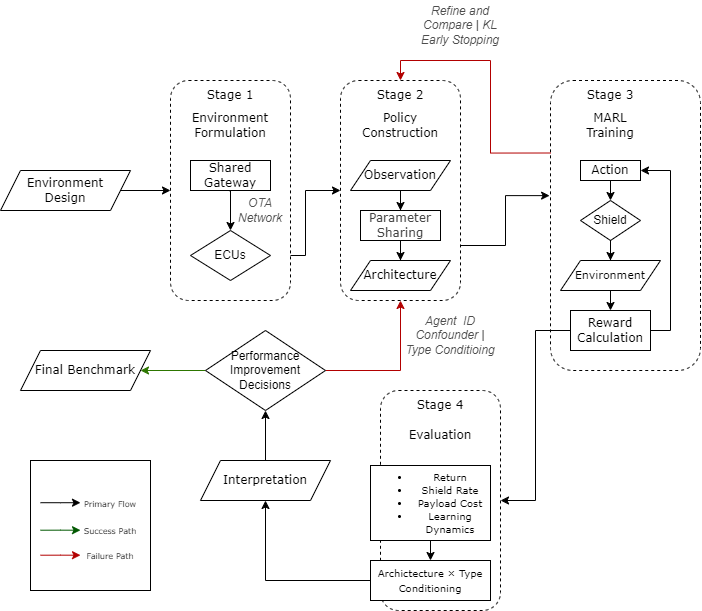
\includegraphics[width=0.96\textwidth]{figures/architecture2.png}
\caption{High-level MA-ReLES-OTA execution and learning loop. Each ECU produces a masked candidate action through IPPO, MAPPO, or FP3O; the shared gateway and cost model determine the physical cost, the safety shield filters unsafe proposals, and Shapley credit assignment distributes the resulting coalition value for PPO updates.}
\label{fig:architecture}
\end{figure}

\section{Problem Formulation}
The environment is represented as a Dec-POMDP
\begin{equation}
\mathcal{M}=\langle\mathcal{S},\{\mathcal{A}_i\}_{i=1}^{N},\mathcal{P},R,\{\Omega_i\}_{i=1}^{N},\mathcal{O},\gamma\rangle,
\end{equation}
where $N$ is the number of ECU agents, $\mathcal{S}$ is the fleet state, $\mathcal{A}_i$ is the action space of ECU $i$, and $\Omega_i$ is its local observation space. At time $t$, agent $i$ receives $o_i^t=\mathcal{O}(s_t,i)$ and chooses $a_i^t$. The joint action is $\mathbf{a}_t=(a_1^t,\ldots,a_N^t)$ and induces a transition under $\mathcal{P}$.

The training objective is the discounted return
\begin{equation}
J(\theta)=\mathbb{E}_{\pi_\theta}\left[\sum_{t=0}^{T-1}\gamma^t r_t\right],\qquad \gamma=0.99.
\end{equation}
Unlike supervised learning, the training data are generated online by the environment. The policy changes the distribution of future observations by changing the sequence of firmware operations, transmission contention, memory usage, and completion times \parencite{sutton2018rl}.

\section{Firmware and Action Model}
Each ECU maintains 16 firmware blocks in the headline experiments. An action is a pair
\begin{equation}
a_i^t=(b_i^t,o_i^t),
\end{equation}
where $b_i^t$ is the selected block and $o_i^t\in\{0,1,2\}$ denotes Copy, Modify, or Modify+Backup (MB). The environment maintains a binary mask indicating which blocks remain. Invalid block selections are suppressed before sampling using action masking, following the policy-gradient action-masking literature \parencite{huang2022masking}.

The underlying cost engine is shared between the legacy single-agent and MARL environments. This design is important because it prevents the single-agent and multi-agent versions from silently using different firmware economics. The current implementation estimates a delta payload from block similarity, applies operation-specific encoding overhead, and then converts payload to a transmission cost using latency, packet loss, and bandwidth factors \parencite{ma_reles_ota_repo}.

\section{Heterogeneous ECU Types}
Four semantic ECU types are used:
\begin{enumerate}[leftmargin=*]
    \item \textbf{Engine:} safety-critical and assigned a relative preference for Modify+Backup.
    \item \textbf{Braking:} safety-critical with a milder preference for Modify+Backup.
    \item \textbf{Infotainment:} non-safety-critical and assigned a preference for Copy.
    \item \textbf{Generic:} neutral baseline with no operation-specific preference.
\end{enumerate}

These preferences are implemented through multiplicative operation costs. The multipliers are deliberately qualitative rather than claims about measured production ECU costs. Their purpose is to create a controlled, reproducible conflict in the optimization problem.

\begin{table}[H]
\centering
\small
\begin{tabular}{lrrr}
\toprule
ECU type & Copy & Modify & Modify+Backup\\
\midrule
Engine & 1.0 & 1.8 & 0.6\\
Braking & 1.0 & 1.2 & 0.8\\
Infotainment & 0.6 & 1.0 & 1.5\\
Generic & 1.0 & 1.0 & 1.0\\
\bottomrule
\end{tabular}
\caption{Operation-specific cost multipliers used to induce controlled qualitative policy conflict. Values below one reduce the relative cost of an operation for that ECU type.}
\label{tab:multipliers}
\end{table}

\section{Observation Space and Type Conditioning}
For each active ECU, the observation contains the remaining-block mask, cumulative encoding cost, cumulative transmission cost, normalized memory usage, step count, ECU-type one-hot vector, and a global state representation used by the centralized critic. In coupled mode, the global state also includes a normalized gateway-load scalar.

The semantic type vector is
\begin{equation}
\mathbf{e}_i\in\{0,1\}^{4},
\end{equation}
with one active component for engine, braking, infotainment, or generic. This vector is intentionally shared by all agents of the same type. It therefore provides role information without providing a unique key for individual agents.

This distinction is essential. A raw \texttt{agent\_id} vector can make the policy memorize fixed agent-specific behavior. Because the experiment assigns a fixed ECU type to each agent, the ID can indirectly reveal the type while simultaneously preserving individual identity. The corrected representation is therefore semantic rather than identifying. This follows the methodological concern raised by Terry et al. regarding agent indication and parameter sharing \parencite{terry2020revisiting}.

\section{Death Masking}
The environment uses variable-length agent episodes because an ECU disappears from active decision making after all of its blocks are processed. To preserve fixed-size tensors for vectorized training, terminated or truncated agents are represented by zeroed local fields while retaining the ECU-type vector. The global state is reconstructed from the fleet and can still indicate which agents are inactive. This is an implementation choice rather than a claim that a terminated ECU is literally in a zero physical state. The exact masking and inactive-agent handling are defined by the repository implementation and therefore constitute an internal source for the reported experimental behavior \parencite{ma_reles_ota_repo}.

The approach is related to variable-length MARL techniques such as those used in CAV-oriented MAPPO variants \parencite{guo2024mappopis}. It also reduces shape changes in the centralized critic and allows the training pipeline to continue using a fixed agent set.

\section{Coupled Gateway Channel}
The major update in the research paper is the introduction of a shared gateway. Let $B_{\mathrm{gw}}$ denote the total gateway downlink capacity and $n_{\mathrm{tx}}$ the number of agents performing transmitting operations in the current step. The effective bandwidth is
\begin{equation}
B_{\mathrm{eff}}=\frac{B_{\mathrm{gw}}}{\max(n_{\mathrm{tx}},1)}.
\label{eq:gateway}
\end{equation}

The primary benchmark uses $B_{\mathrm{gw}}=25$ Mbps. This is a scenario parameter, not a claim that every production vehicle gateway operates at exactly 25 Mbps. GSMA deployment guidance reports experienced downlink rates of 50 Mbps in several 5G scenarios, including urban and high-speed-vehicle cases, making a 25 Mbps shared-gateway scenario a deliberately constrained operating point \parencite{gsma2019fiveg}.

Only Modify and Modify+Backup count toward $n_{\mathrm{tx}}$. Copy is exempt because the implementation treats its approximately 64-byte delta as a negligible control-plane operation rather than a data-plane firmware transfer \parencite{ma_reles_ota_repo}. This is a modelling assumption and should not be interpreted as a universal property of every automotive OTA stack.

\section{Stochastic Channel Model}
The transmission-cost engine uses a truncated Gaussian latency model with a nominal mean of 120 ms and support from 50 to 200 ms. Packet-loss and bandwidth factors are combined with payload size to form the transmission cost \parencite{ma_reles_ota_repo}. This stochasticity prevents the policy from solving only one deterministic channel realization and is consistent with the broader motivation for learning under uncertain environment dynamics \parencite{sutton2018rl}.

The repository currently centralizes these physical parameters in \texttt{ota\_core.py} and the configuration module \parencite{ma_reles_ota_repo}. Because some older command-line defaults remain in legacy training scripts, the thesis treats the experiment paper and the final experiment runner as the authoritative description of the reported benchmark, while the appendix records the implementation parameters needed for reproduction.

\section{Reward and Shapley Credit Assignment}\label{sec:reward}
The environment first evaluates the joint coalition value. A simplified form is
\begin{equation}
v(S)=\sum_{j\in S\setminus\mathcal{S}_{\mathrm{shield}}}
\left[-\alpha(C_{\mathrm{enc}}^j+C_{\mathrm{tx}}^j)m_j-\beta O_j+10\,\mathbb{I}(\mathrm{Complete}_j)\right],
\end{equation}
where $m_j$ is the type-operation multiplier, $O_j$ is operation overhead, and $\alpha$ and $\beta$ keep the reward numerically manageable. Valid progress receives an additional dense progress bonus. Invalid actions and step-limit violations receive explicit penalties, while a shielded action receives zero task reward because the proposed action was not actually executed.

For agent $i$, the Shapley value is
\begin{equation}
\phi_i(v)=\frac{1}{N!}\sum_{\pi\in\Pi}\left[v(P_i^\pi\cup\{i\})-v(P_i^\pi)\right],
\end{equation}
where $P_i^\pi$ is the set of agents preceding $i$ in permutation $\pi$ \parencite{shapley1953value}. Since the headline experiments use four agents, all 24 permutations can be enumerated exactly. For larger fleets, the same formulation can be approximated through sampling, following sampling-based Shapley computation \parencite{castro2009shapley}.

Shapley credit assignment is not claimed to make the learning problem perfectly independent across agents. Its purpose is to reduce the arbitrariness of assigning a joint cost to individual policies when the actions have heterogeneous marginal contributions, following the cooperative-game interpretation of marginal contribution \parencite{shapley1953value,castro2009shapley}. The specific coalition construction and reward implementation used in this thesis are internal to the MA-ReLES-OTA environment \parencite{ma_reles_ota_repo}.

\section{Safety Shield}
The safety layer is a deterministic runtime filter inspired by the general idea of reinforcement-learning shields \parencite{alshiekh2018shielding} and by Control Barrier Function safety reasoning \parencite{ames2019cbf}. The implementation checks proposed joint memory overhead against a fleet-level safety limit. When the proposed coalition would violate the limit, actions with the largest overhead are blocked in greedy order until the constraint is satisfied.

The nominal safety threshold is 85\% of the configured memory budget. The shield is therefore an external safety mechanism rather than a reward-only penalty. This makes it possible to measure \emph{shield intervention rate} as a behavioral metric. A policy with high return but frequent shield interventions is operationally different from one that naturally proposes actions that satisfy the constraint.

The thesis deliberately avoids calling the implementation a formally verified CBF controller. The CBF literature motivates the conceptual separation between performance optimization and safety enforcement, but the actual filter is a discrete, application-specific rule set.

\section{Policy Architectures}\label{sec:architectures}
All three algorithms use PPO as the optimization backbone \parencite{schulman2017ppo}.

\subsection{IPPO}
IPPO uses a shared actor representation and independent PPO learning across the agents. In the type-conditioned configuration, the same actor receives the ECU-type vector and can therefore learn a conditional policy $\pi(a\mid o, e)$. In the blind configuration, the type vector is removed.

\subsection{MAPPO}
MAPPO uses the same basic actor representation as the shared IPPO condition but provides a centralized critic with access to the joint state during training. This follows the CTDE design that has been shown to be a strong cooperative MARL baseline \parencite{yu2022surprising}.

\subsection{FP3O}
FP3O uses a shared backbone followed by type-specific policy heads. The implementation uses a three-layer backbone with widths $256\rightarrow256\rightarrow128$ and separate action and position heads for the four ECU types. A centralized critic is retained. Thus, FP3O shares lower-level representation parameters but reduces parameter sharing at the final action-distribution stage \parencite{feng2023fp3o}.

The key representational distinction is
\begin{equation}
\theta_{\mathrm{shared}}=\{\theta_{\mathrm{backbone}},\theta_{\mathrm{head}},\theta_{\mathrm{critic}}\}
\end{equation}
for a fully shared actor, versus
\begin{equation}
\theta_{\mathrm{FP3O}}=\left\{\theta_{\mathrm{backbone}},\{\theta_{\mathrm{head}}^k\}_{k\in\mathcal{K}},\theta_{\mathrm{critic}}\right\}
\end{equation}
for type-specialized heads.

\section{Optimization and Numerical Stability}
The PPO objective uses the clipped policy ratio
\begin{equation}
\mathcal{L}^{\mathrm{CLIP}}(\theta)=\hat{\mathbb{E}}_t\left[\min\left(r_t(\theta)\hat A_t,\operatorname{clip}(r_t(\theta),1-\epsilon,1+\epsilon)\hat A_t\right)\right],
\end{equation}
where $\epsilon=0.2$ and the advantage is estimated with GAE using $\gamma=0.99$ and $\lambda=0.95$ \parencite{schulman2017ppo,schulman2015trpo}.

Training uses Adam \parencite{kingma2015adam}, multiple parallel environments, gradient clipping, reward normalization through Stable-Baselines3's \texttt{VecNormalize}, and a target-KL stopping threshold in the final runner. Earlier development experimented with adaptive value normalization inspired by PopArt \parencite{hessel2019popart}; the current repository instead uses the native \texttt{VecNormalize} mechanism and clamps policy logits to a finite range. These changes were introduced after numerical instability and NaN-producing updates appeared during high-penalty training.

The important methodological point is that stabilization measures are applied consistently across the compared algorithms. The study does not tune the numerical pipeline separately to rescue one architecture.


\section{Design Assumptions and Scope}
The environment is intentionally positioned between a purely abstract MARL benchmark and a production automotive simulator. The objective is not to reproduce every component of a commercial OTA platform. Instead, the model retains the decision variables that are necessary for studying the research question: which firmware block is selected, which update operation is applied, how much communication cost is incurred, how concurrent transmissions affect a shared gateway, and when a proposed action must be filtered because of a fleet-level resource constraint. This scoped design makes it possible to attribute changes in behavior to representation and coupling choices without introducing a large number of uncontrolled protocol variables.

Several assumptions follow from this choice. First, firmware blocks are treated as independently selectable decision units within an ECU backlog. This does not imply that real firmware images are always semantically decomposable in this way. It provides a repeatable action structure with which masking and heterogeneous operation costs can be studied. Second, the operation multipliers are synthetic experimental parameters. They encode qualitative differences among ECU roles rather than measurements taken from a particular vehicle platform. Third, the gateway model represents contention at the level of available transmission capacity. It is therefore a scheduling abstraction, not a complete model of cellular, Ethernet, CAN, or UDS timing. These boundaries are important because the thesis claims concern the controlled optimization problem implemented in MA-ReLES-OTA.

The same distinction applies to safety. Automotive functional safety and diagnostic standards provide important context for why update procedures cannot be evaluated only by transfer cost \parencite{iso26262,iso14229}. However, compliance with those standards is outside the scope of the simulator. The rule-based shield is an experimental safety mechanism that prevents a specified memory condition from being violated. Its role is to create a measurable separation between what the learned policy proposes and what the environment ultimately permits. Consequently, shield rate is interpreted as evidence about learned constraint awareness, not as a certification result.

\section{Comparability Across Architectures}
A central experimental requirement is that architectural comparisons must not silently compare different tasks. All algorithmic conditions therefore operate on the same firmware backlog structure, cost engine, action masking rules, reward accounting, stochastic channel family, and termination semantics. The architecture changes how policy and value representations are organized, while conditioning changes what semantic information is supplied to the policy. This separation is necessary because a result cannot be attributed to specialization if specialized agents also receive information that shared agents never observe.

The identity-confound experiment motivated an additional comparability rule. An observation feature is not treated as harmless merely because it is numerically simple. A stable agent identifier can encode role information whenever the mapping between identity and role is fixed. Under parameter sharing, the network can then learn identity-specific behavior while the experiment is described as using a common policy. The corrected design therefore uses semantic type vectors when role information is intended and avoids raw identifiers as substitutes. This follows the broader observation that parameter sharing and agent indication must be interpreted together rather than as independent implementation details \parencite{terry2020revisiting}.

The comparison also distinguishes early-training performance from long-horizon performance. PPO-based algorithms can exhibit different transient learning dynamics even when they eventually approach similar returns. Reporting only a final converged score can hide a practically relevant difference in sample efficiency, while reporting only an early checkpoint can overstate a difference that disappears with further training. The two horizons used in this thesis therefore answer different questions. The approximately 100k-step experiment describes behavior under a fixed, limited training budget. The approximately 2.0M-step validation asks whether the observed ordering persists after substantially more optimization. This distinction is consistent with the need to evaluate both learning dynamics and final policy quality in empirical MARL studies \parencite{yu2022surprising,raffin2021sb3}.

\section{Development Lifecycle}
The research progressed through the following stages:
\begin{enumerate}[leftmargin=*]
    \item Single-agent ReLES-OTA reproduction and validation of the shared cost engine.
    \item PettingZoo multi-agent conversion with variable-length agents and stochastic channels.
    \item Safety shielding, action masking, Shapley credit assignment, and numerical stabilization.
    \item ECU heterogeneity through operation-specific cost multipliers.
    \item Discovery of the \texttt{agent\_id} confound and replacement with semantic \texttt{ecu\_type} conditioning.
    \item Fair isolated-channel comparison of shared and specialized policies.
    \item Introduction of shared gateway contention and Copy exemption.
    \item Five-seed coupled-channel benchmark followed by long-horizon validation.
\end{enumerate}

This lifecycle is important because the final coupled-channel result is not a single isolated experiment. It is the endpoint of a sequence in which earlier negative or inconclusive results motivated controlled changes to the environment and observation design.

\chapter{Experimental Design and Results}


\section{Experimental Protocol and Evaluation Procedure}
Each configuration is trained from independently initialized random seeds. A seed controls the stochastic elements of initialization and environment sampling, so repeated runs provide a distribution of outcomes rather than a single potentially lucky trajectory. This repeated-seed approach is particularly important for policy-gradient experiments because stochastic initialization and rollout sampling can materially affect observed training outcomes \parencite{schulman2017ppo,raffin2021sb3}. For every run, the same training budget and configuration are maintained within the corresponding experimental matrix. The reported mean return is then interpreted together with variability across seeds rather than as a deterministic property of an algorithm.

The primary metric is episodic return, where a larger value corresponds to lower accumulated update cost under the reward formulation. Return alone is insufficient because a policy can obtain a favorable executed trajectory while repeatedly proposing actions that are later corrected by the shield. The evaluation therefore records the fraction of decision points at which the shield intervenes. A low intervention rate indicates that the policy's proposals more often satisfy the environment's resource condition before correction. It does not prove that the policy is safe in states not represented by the simulator, and it should not be confused with a formal safety certificate.

Payload-related cost is reported as a complementary operational measure. This helps distinguish a return change caused by the communication and encoding economics from one caused primarily by other reward components. Where appropriate, the analysis also compares seed-level returns using Welch's t-test because the sample variances need not be assumed equal. A non-significant result is not interpreted as evidence that two algorithms are identical. It means that the available sample does not provide sufficient evidence for a difference under the chosen test and significance threshold.

The staged design is also part of the evaluation protocol. Earlier stages are not pooled numerically with the coupled-channel benchmark because they represent different environment regimes. Instead, they are used to explain how the final experiment was reached. Homogeneous settings establish a baseline in which specialization should have little role-specific information to exploit. Structural heterogeneity introduces conflicting preferences. The identity-confound stage tests whether the observation itself can create hidden specialization. Isolated semantic conditioning then establishes what a shared network can do when explicit role information is available. Finally, the coupled gateway introduces the physical interaction that makes one agent's transmission behavior directly affect the others.

\section{Statistical Reporting Principles}
The thesis follows several conservative rules when converting experimental measurements into claims. First, the mean is never treated as sufficient evidence by itself when seed variability is large. Second, confidence intervals and seed dispersion are reported to show uncertainty in the estimate. Third, a result with a lower mean but a lower shield rate may still represent an attractive engineering trade-off, so the discussion keeps reward and safety behavior separate. Fourth, the absence of statistical significance is not rewritten as proof of equivalence. Finally, causal language is restricted to mechanisms that are actually observed in the implementation.

This last rule is especially relevant to the term \emph{Representation Interference}. The measured result is an interaction between architecture and type conditioning: adding type information changes the algorithms in different directions. The thesis does not record gradients, feature activations, or optimization conflicts that would establish a neural mechanism. The term therefore names a behavioral pattern observed at the system level. This wording preserves the explanatory value of the pattern while preventing an unsupported claim about internal gradient dynamics.

\section{Experimental Matrix}
The primary benchmark uses four agents, 16 firmware blocks per agent, a 25 Mbps coupled gateway, stochastic channel conditions, and an 85\% fleet-memory safety threshold. The architecture-by-conditioning matrix is:
\begin{table}[H]
\centering
\small
\begin{tabular}{lll}
\toprule
Architecture & Blind & Type-conditioned\\
\midrule
IPPO & Yes & Yes\\
MAPPO & Yes & Yes\\
FP3O & Yes & Yes\\
\bottomrule
\end{tabular}
\caption{Primary $2\times3$ factorial design. ``Blind'' removes the semantic ECU-type vector; ``Type-conditioned'' supplies the four-dimensional ECU-type representation.}
\label{tab:matrix}
\end{table}

The updated research paper treats 100,353 timesteps per seed as the primary transient benchmark and 2,000,897 timesteps as the long-horizon validation. Five independent seeds are used for each configuration. Means and 95\% confidence intervals are computed over seed-level evaluation returns, and Welch's unequal-variance $t$-test is used for pairwise comparisons.

\section{Staged Experimental Findings}

\subsection{Stage 1: Homogeneous Environment}
In the homogeneous stage, ECU type labels do not create meaningful differences in the reward or cost structure. The earlier experiments showed that shared policies were already competitive, with IPPO/MAPPO around 12.85 mean return versus approximately 11.44 for FP3O. This result is unsurprising: if the agents have no meaningful role difference, specialized heads divide training data without providing a corresponding representational benefit. The observation is consistent with the broader evidence that simple shared PPO policies can be highly effective in cooperative MARL \parencite{yu2022surprising}.

\subsection{Stage 2: Uniform Heterogeneity}
A second stage varied the magnitude of costs without changing the ordering of preferred operations. This did not create a qualitative policy conflict: all ECU types still preferred essentially the same operation ranking. The experiment therefore demonstrated an important design lesson. A numerical difference in cost is not necessarily sufficient to test heterogeneous policy representation; the environment must create different preferred behaviors.

\subsection{Stage 3: Structural Heterogeneity and the Identity Confound}
The third stage introduced the operation-specific multipliers in Table~\ref{tab:multipliers}. Engine and braking roles were made relatively more favorable toward Modify+Backup, while infotainment was made relatively more favorable toward Copy. This created a genuine qualitative conflict.

However, the initial observation design included a unique \texttt{agent\_id}. Because the mapping from agent ID to ECU type was fixed, a shared policy could infer the role from the ID while also retaining a unique representation for every individual agent. The resulting architecture was therefore not a clean test of semantic parameter sharing. This observation agrees with the warning in the parameter-sharing literature that agent indication can fundamentally change what a shared network can represent \parencite{terry2020revisiting}.

The experiment was consequently redesigned rather than treated as evidence for either hypothesis.

\subsection{Stage 4: Semantic Type Conditioning in Isolated Channels}
After replacing \texttt{agent\_id} with \texttt{ecu\_type}, the isolated-channel experiment provided a much fairer test. In the authoritative five-seed isolated benchmark recorded in the project artifacts, IPPO and MAPPO both achieved approximately 16.71 mean return with extremely small confidence intervals, whereas FP3O averaged approximately 5.09 with a wide interval dominated by one failed seed. FP3O's five seed returns were $\{15.09,15.18,10.85,16.71,-32.37\}$.

This result established an important baseline: explicit specialization is not automatically beneficial merely because the agents are heterogeneous. If the channel remains effectively separable, a shared policy with semantic type information can be highly competitive. It also motivated the question addressed by the updated paper: whether the conclusion changes when the communication resource itself becomes coupled.

\section{Primary Coupled-Channel Benchmark}
Table~\ref{tab:coupled} gives the updated five-seed benchmark generated by the project experiment pipeline \parencite{ma_reles_ota_repo}. The central result is not simply the ranking of the six rows, but the interaction between architecture and type conditioning.

\begin{table}[H]
\centering
\scriptsize
\begin{tabular}{llrrrr}
\toprule
Algorithm & Condition & Return & CI$_{95}$ & Shield (\%) & Payload (B)\\
\midrule
IPPO & Blind & \textbf{-85.27} & 173.39 & 32.66 & \textbf{78,239.5}\\
IPPO & Type & -112.64 & 160.46 & 32.40 & 91,953.5\\
MAPPO & Blind & -135.70 & 172.42 & 48.41 & 98,363.8\\
MAPPO & Type & -187.88 & 142.02 & 64.99 & 118,218.5\\
FP3O & Blind & -213.64 & 69.75 & 64.68 & 131,782.3\\
FP3O & Type & -102.20 & 113.58 & \textbf{13.82} & 106,121.9\\
\bottomrule
\end{tabular}
\caption{Authoritative coupled-channel factorial benchmark: five seeds, 100,353 timesteps per seed, four agents, 16 blocks per agent, and a 25 Mbps shared gateway. CI values are half-widths. Higher return (less negative) is better; lower shield intervention and payload are better.}
\label{tab:coupled}
\end{table}

\begin{figure}[H]
\centering
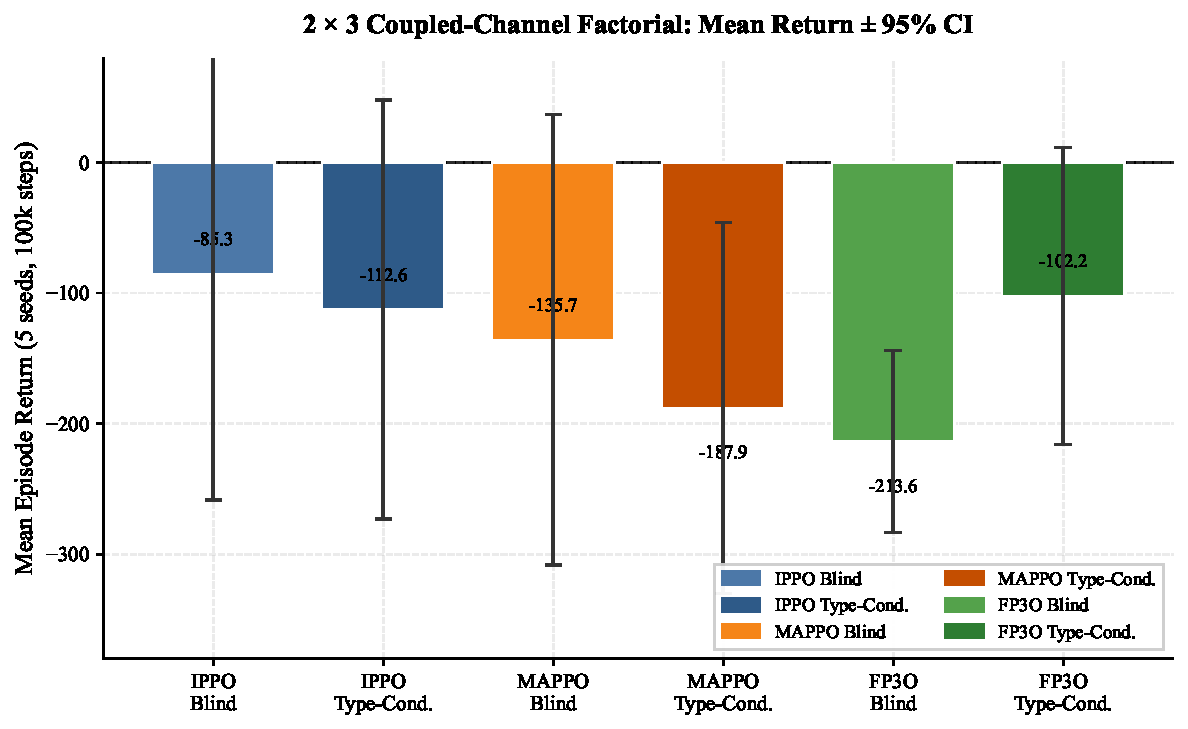
\includegraphics[width=0.98\textwidth]{figures/fig_coupled_comparison.pdf}
\caption{Mean return with 95\% confidence intervals for the six coupled-channel architecture-by-conditioning configurations. The most important pattern is the directional reversal caused by type conditioning: the shared IPPO and MAPPO rows decline, while FP3O improves strongly.}
\label{fig:coupledcomparison}
\end{figure}

The primary benchmark in Table~\ref{tab:coupled} summarizes the endpoint performance of the six configurations, but it does not by itself show how the policies arrived at those outcomes during training. This distinction is important in on-policy reinforcement learning because the reported endpoint depends on the trajectory distribution generated during optimization rather than on a fixed supervised dataset \parencite{sutton2018rl,schulman2017ppo}. The following two diagnostics therefore examine the learning process in the same coupled-channel setting. They are interpreted as training-dynamics evidence and are not used to replace the authoritative five-seed benchmark.

\begin{figure}[H]
\centering
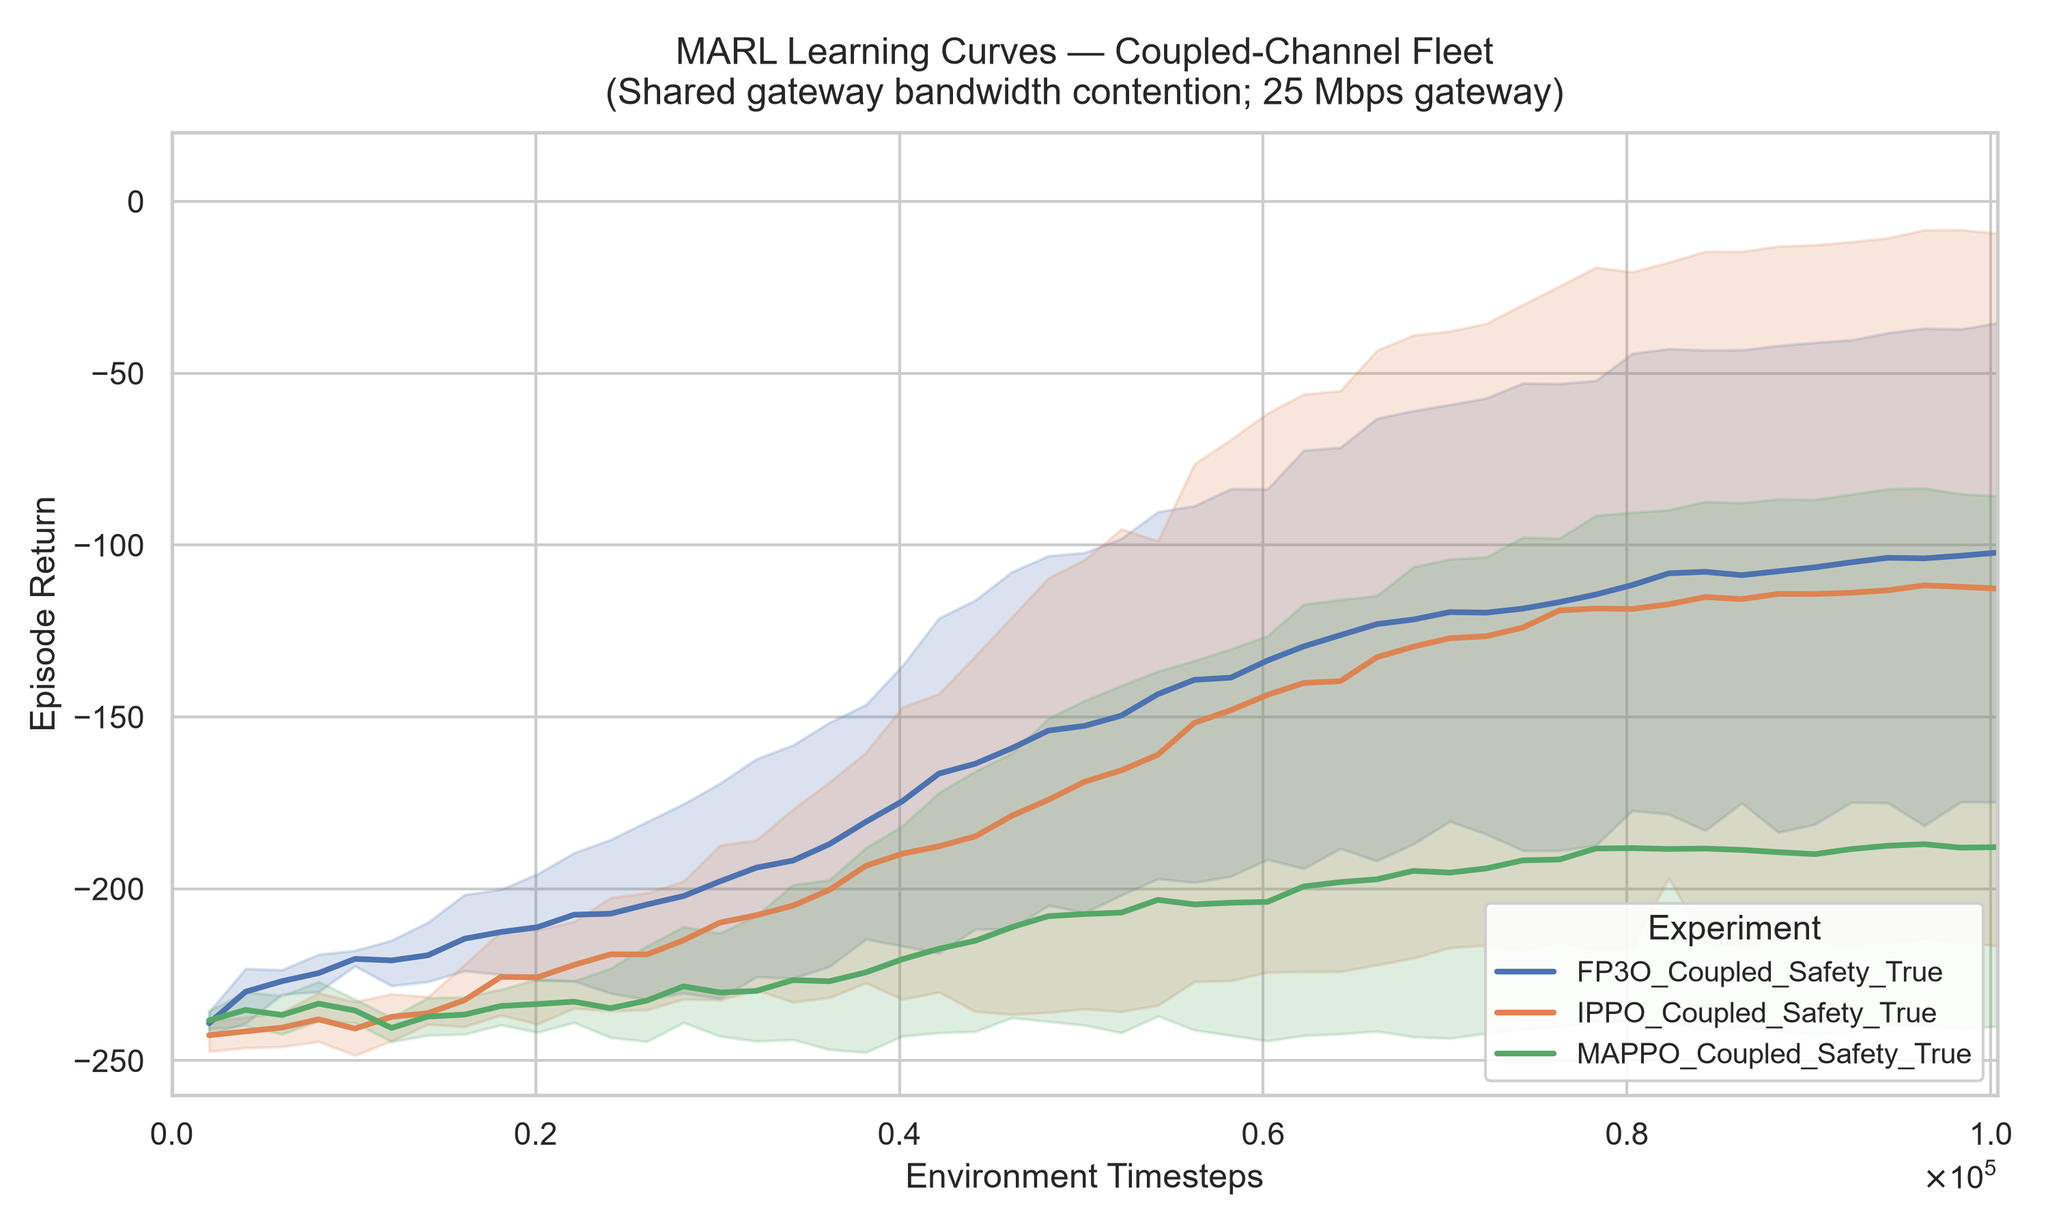
\includegraphics[width=0.98\textwidth]{figures/coupled_channel_learning_curves.png}
\caption{Training learning curves for the coupled-channel fleet under a 25 Mbps shared gateway. The curves show the progression of episode return for FP3O, IPPO, and MAPPO with the safety mechanism enabled. The shaded regions indicate the observed variability around the plotted training trajectories.}
\label{fig:coupledlearning}
\end{figure}

Figure~\ref{fig:coupledlearning} provides a direct view of the early training behavior that is compressed into the aggregate values reported in Table~\ref{tab:coupled}. All three methods improve substantially from their initial returns, but the rate and stability of improvement differ. FP3O and IPPO move toward substantially less negative returns as training proceeds, whereas MAPPO improves more gradually and remains below the other two methods at the end of the displayed training horizon. The relatively broad uncertainty regions are also important: they show that the training process is not deterministic and that intermediate performance should not be interpreted as a precise estimate of the final policy quality.

The figure is particularly useful for interpreting the 100,353-timestep benchmark. The endpoint of a learning curve can be affected by the optimization stage reached at the selected training budget. Consequently, a difference between algorithms at approximately 100k timesteps may reflect differences in learning speed, exploration, or convergence behavior rather than a difference in the best policy that each algorithm could eventually obtain. This is consistent with the separate long-horizon validation reported later in this chapter, where the reward signal becomes substantially less discriminative.

\begin{figure}[H]
\centering
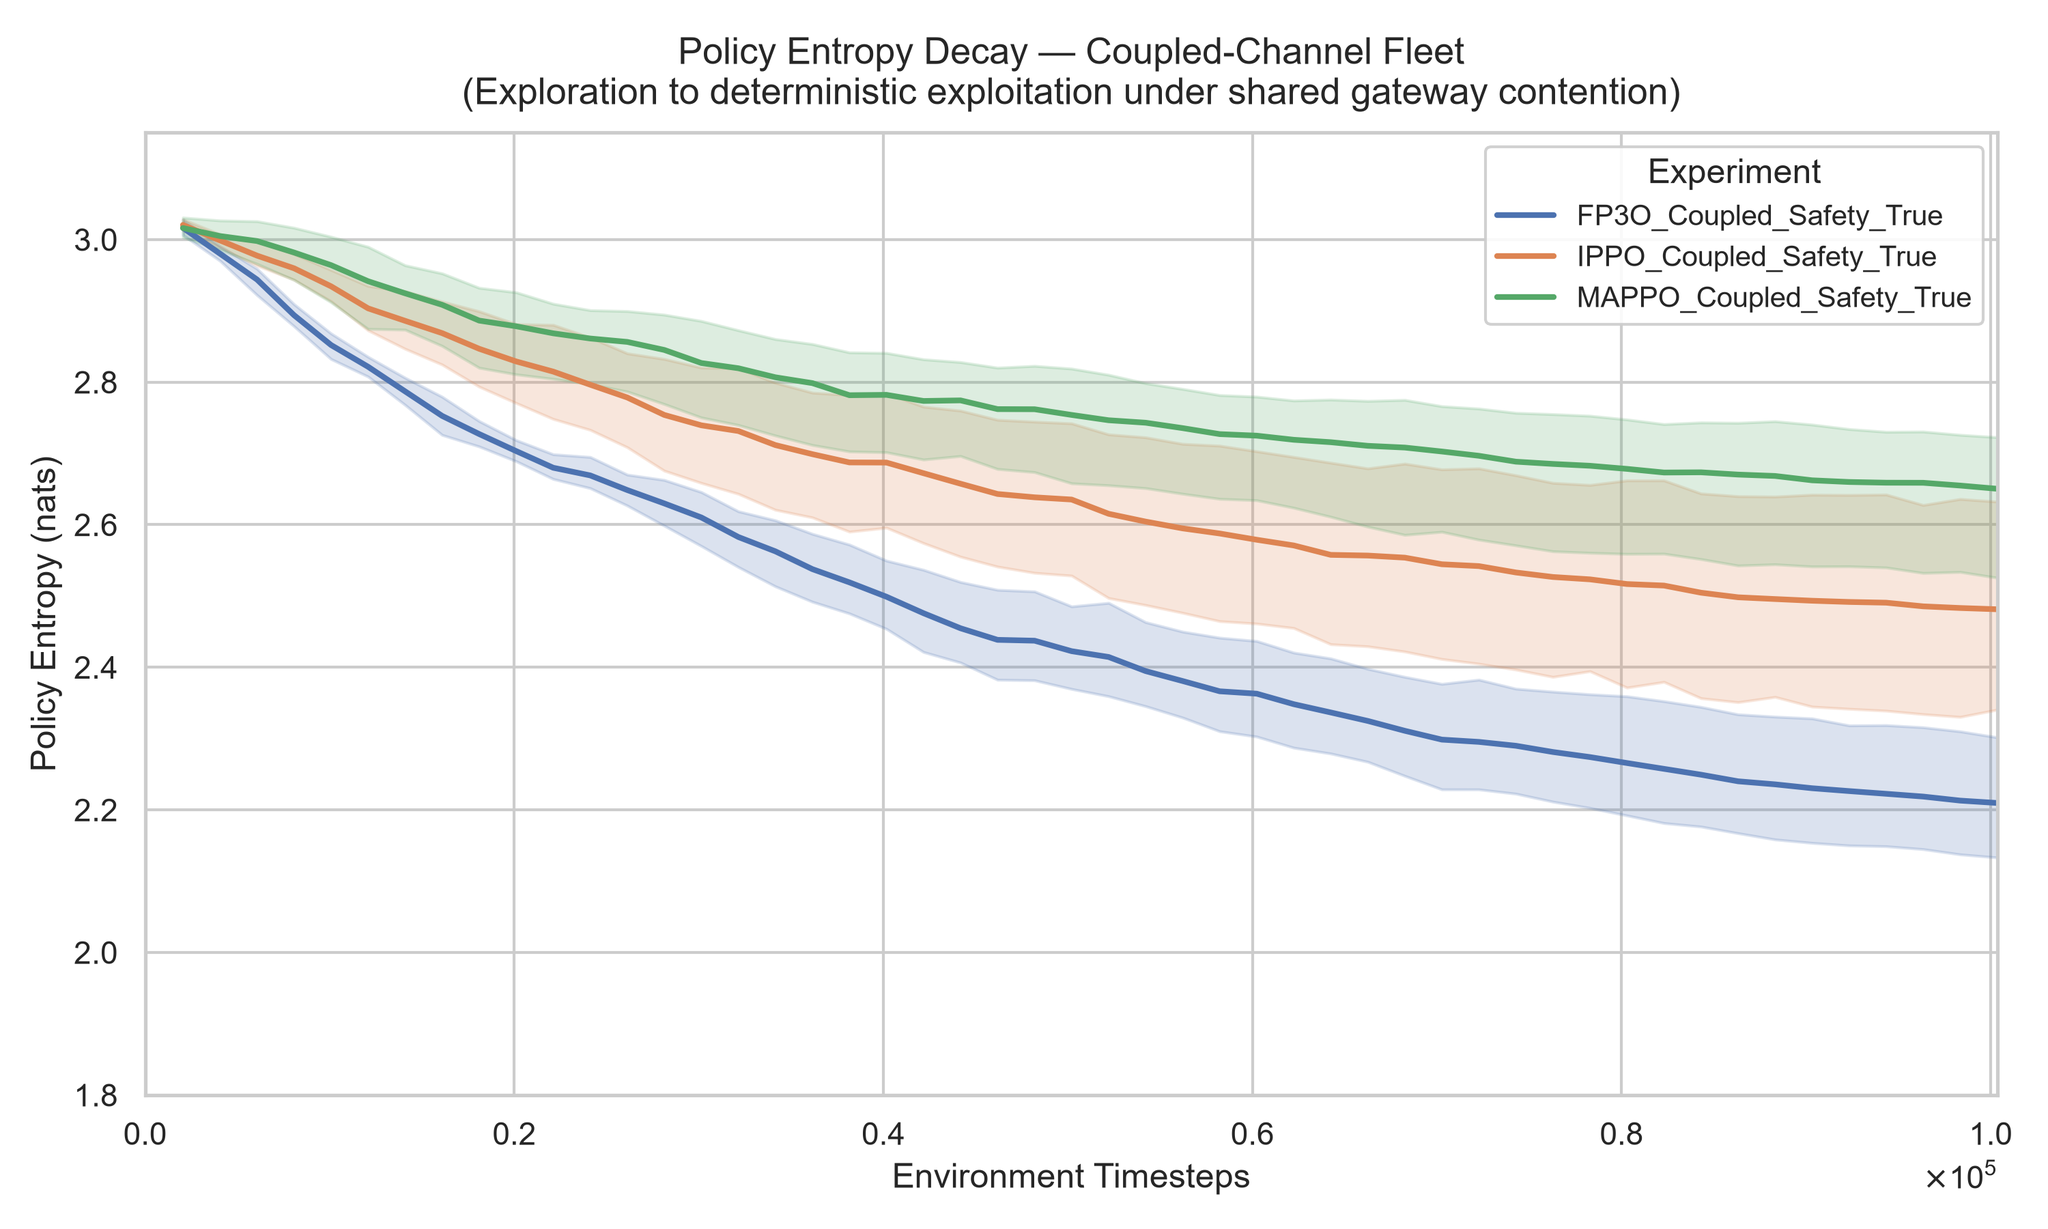
\includegraphics[width=0.98\textwidth]{figures/coupled_channel_policy_entropy_decay.png}
\caption{Policy entropy during coupled-channel training under a shared 25 Mbps gateway. The decreasing entropy indicates a gradual transition from broader exploration toward more concentrated action selection for FP3O, IPPO, and MAPPO.}
\label{fig:coupledentropy}
\end{figure}

Figure~\ref{fig:coupledentropy} complements the return curves by showing the evolution of policy uncertainty. All three algorithms begin with entropy close to 3.0 nats and gradually decrease their entropy during training. FP3O exhibits the strongest reduction, reaching approximately 2.2 nats by the end of the displayed horizon, while IPPO and MAPPO retain higher entropy. This indicates that FP3O becomes more concentrated in its action selection under the coupled-channel constraint, whereas the shared-policy methods continue to preserve comparatively broader action distributions.

The entropy curves should not be interpreted as evidence that lower entropy is inherently better. Exploration is necessary during learning, and a policy can become prematurely deterministic without discovering a high-quality strategy. In the present study, entropy is therefore treated as a diagnostic that helps explain the training trajectories rather than as an independent optimization objective. Considered together with the return curves, the figure suggests that the algorithms differ not only in their achieved returns but also in how quickly their policies transition from exploration toward exploitation.

\section{Representation Interference Pattern}
Type conditioning changes IPPO from $-85.27$ to $-112.64$, a 27.4-point decrease, and changes MAPPO from $-135.70$ to $-187.88$, a 52.2-point decrease. FP3O changes in the opposite direction, from $-213.64$ to $-102.20$, an improvement of 111.44 points.

We call this behavioral pattern \emph{Representation Interference}. The interpretation is that a single shared actor is being asked to encode role-dependent responses under a coupled communication constraint, while its parameter updates remain shared across all roles. This is conceptually related to gradient conflict in multi-task learning \parencite{yu2020pcgrad}, but the present experiments do not record or compare per-type gradient vectors. Therefore, ``Representation Interference'' is a description of the observed architecture-by-conditioning behavior, not a direct measurement of gradient cancellation.

\begin{figure}[H]
\centering

\includegraphics[width=0.82\textwidth]{figures/fig_interference.pdf}
\caption{Change in mean return when semantic type conditioning is enabled. Negative values occur for IPPO and MAPPO; FP3O exhibits a large positive change. The figure is a behavioral diagnostic and does not directly measure gradients.}
\label{fig:interference}
\end{figure}

\section{Safety-Shield Intervention}
Return alone does not fully capture the engineering quality of an OTA policy. In the primary benchmark, IPPO Blind obtains the best mean return, but its shield intervention rate is 32.66\%. FP3O Type-conditioned has a slightly lower mean return but the lowest intervention rate at 13.82\%.

The difference is operationally meaningful. A shielded action is one that the learned policy proposed but the external safety layer refused to execute. Frequent interventions therefore indicate greater dependence on the external governor. We use ``shield-dependent'' as an operational description only; it does not imply that the policy intentionally exploits the shield.

\begin{figure}[H]
\centering

\includegraphics[width=0.82\textwidth]{figures/fig_shield_rate.pdf}
\caption{Safety-shield intervention rates in the primary five-seed, 100k-step coupled-channel benchmark. FP3O Type-conditioned has the lowest intervention rate among the six configurations.}
\label{fig:shield}
\end{figure}

IPPO Blind and FP3O Type-conditioned have overlapping confidence intervals, and the reported pairwise test does not establish a statistically significant return difference. Consequently, the thesis does not claim that FP3O Type-conditioned is statistically superior in raw return. Instead, it is selected as the preferred operating point under a multi-objective engineering criterion that considers both return and reliance on the safety mechanism.

\section{Payload Cost}
The fleet payload values in Table~\ref{tab:coupled} show a second trade-off. IPPO Blind has the lowest mean payload among the six configurations, while FP3O Type-conditioned reduces payload relative to FP3O Blind but does not become the overall payload minimum.

\begin{figure}[H]
\centering
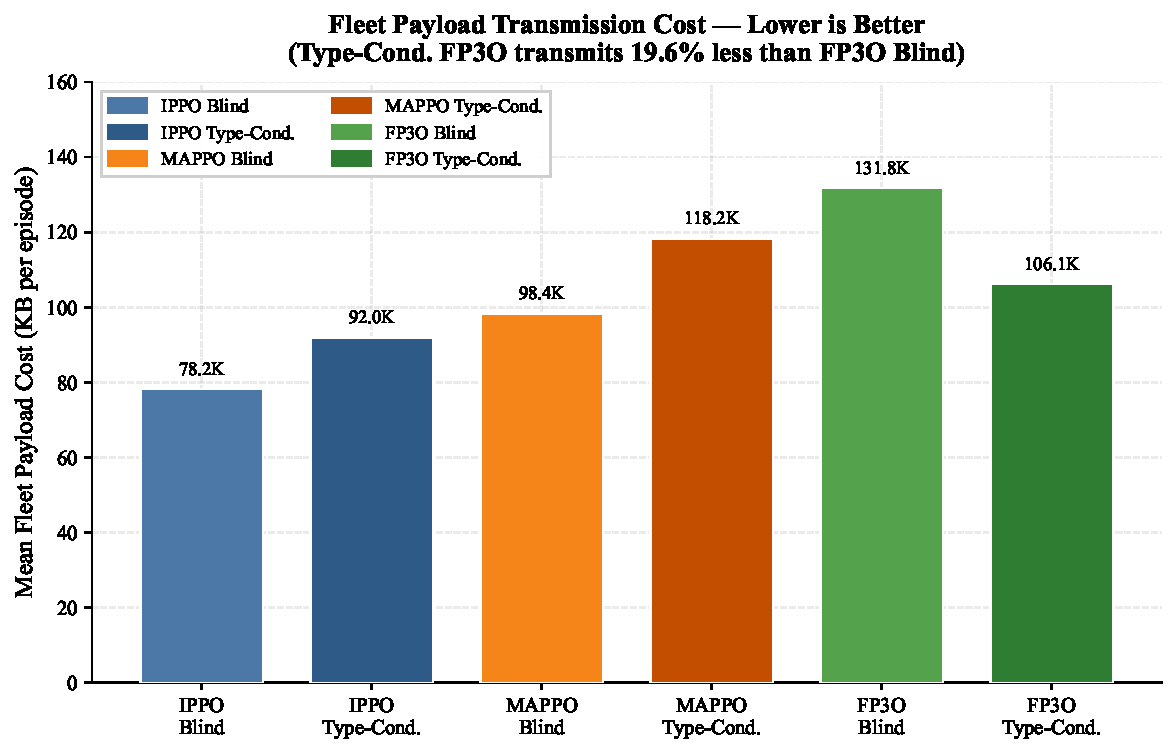
\includegraphics[width=0.88\textwidth]{figures/fig_coupled_payload.pdf}
\caption{Mean fleet payload transmission cost per episode in the updated coupled-channel benchmark. The figure highlights the payload trade-off across the six configurations.}
\label{fig:coupledpayload}
\end{figure}

The project retains a deployment-oriented target of approximately 5,000 bytes as a design objective. The observed payload costs remain substantially above this target, so the current policies should not be interpreted as production-ready OTA schedulers. The payload target is useful as an engineering benchmark, not as a claim derived from a universal automotive standard.

\section{Long-Horizon Validation}
The primary 100,353-step benchmark is intentionally paired with a much longer validation horizon. After 2,000,897 timesteps, all six coupled-channel configurations approach an empirical reward ceiling near 16.71. These values are internal experimental observations from the project runs rather than externally established performance limits \parencite{ma_reles_ota_repo}.

This result changes the interpretation of the short-horizon comparison. It would be incorrect to describe the 100k results as evidence that one architecture has a permanently better asymptotic optimum. Instead, the short-horizon benchmark reveals differences in early training dynamics, coordination, and safety-shield reliance. With sufficient additional optimization, the return signal saturates and becomes less discriminative.

\begin{table}[H]
\centering
\small
\begin{tabular}{lr}
\toprule
Configuration & Long-horizon return\\
\midrule
IPPO Blind & $\approx16.71$\\
IPPO Type-conditioned & $\approx16.71$\\
MAPPO Blind & $\approx16.71$\\
MAPPO Type-conditioned & $\approx16.71$\\
FP3O Blind & $\approx16.71$\\
FP3O Type-conditioned & $\approx16.71$\\
\bottomrule
\end{tabular}
\caption{Long-horizon coupled-channel validation after 2,000,897 timesteps per configuration. Values indicate the empirical reward ceiling observed in the project runs.}
\label{tab:longhorizon}
\end{table}

\begin{figure}[H]
\centering
\includegraphics[width=0.94\textwidth]{figures/fig_reward_saturation.pdf}
\caption{Reward saturation and horizon-dependent masking in the coupled-channel benchmark. Panel (A) shows the full training horizon, where the evaluated policies eventually approach a common empirical reward ceiling. Panel (B) contrasts the approximately 100k-step regime with the 2,000,897-step saturation regime. The comparison illustrates why the shorter benchmark is informative about early training dynamics and safety-shield reliance, whereas the long-horizon result should not be interpreted as evidence of persistent asymptotic differences.}
\label{fig:reward_saturation}
\end{figure}

The reward-saturation diagnostic provides a visual explanation for the distinction between transient and asymptotic performance in the coupled-channel experiment. At approximately 100,000 training steps, the configurations remain separated and the differences in mean return are accompanied by markedly different safety-shield intervention rates. With continued training beyond one million steps, these return differences progressively diminish as the policies approach the same empirical ceiling. This does not invalidate the short-horizon benchmark. Rather, it indicates that the two evaluation horizons measure different properties of the learning process: the shorter horizon exposes how efficiently each architecture learns a useful coordination strategy under a limited training budget, while the longer horizon examines whether those differences remain after substantially more optimization. The figure therefore supports the thesis decision to report both horizons instead of relying on a single final score.

In particular, the diagnostic should not be read as evidence that all configurations are equivalent at every point during training. The 100k-step panel shows that the ordering and safety behavior can differ substantially before saturation. Similarly, the common long-horizon ceiling does not establish that the learned policies are behaviorally identical, because equal aggregate return can still arise from different action distributions, shield usage, or update trajectories. The figure is consequently used as a convergence diagnostic that complements, rather than replaces, the seed-level statistical benchmark and safety analysis.

\section{Earlier Isolated-Channel Training Diagnostics}
The thesis also retains the learning-curve and entropy figures from the earlier isolated-channel, safety-constrained benchmark. These figures are included as historical diagnostic evidence rather than as the primary result. They are useful because they show that the specialized FP3O policy exhibited elevated training-time variance before the coupled-channel experiment was introduced.

\begin{figure}[H]
\centering
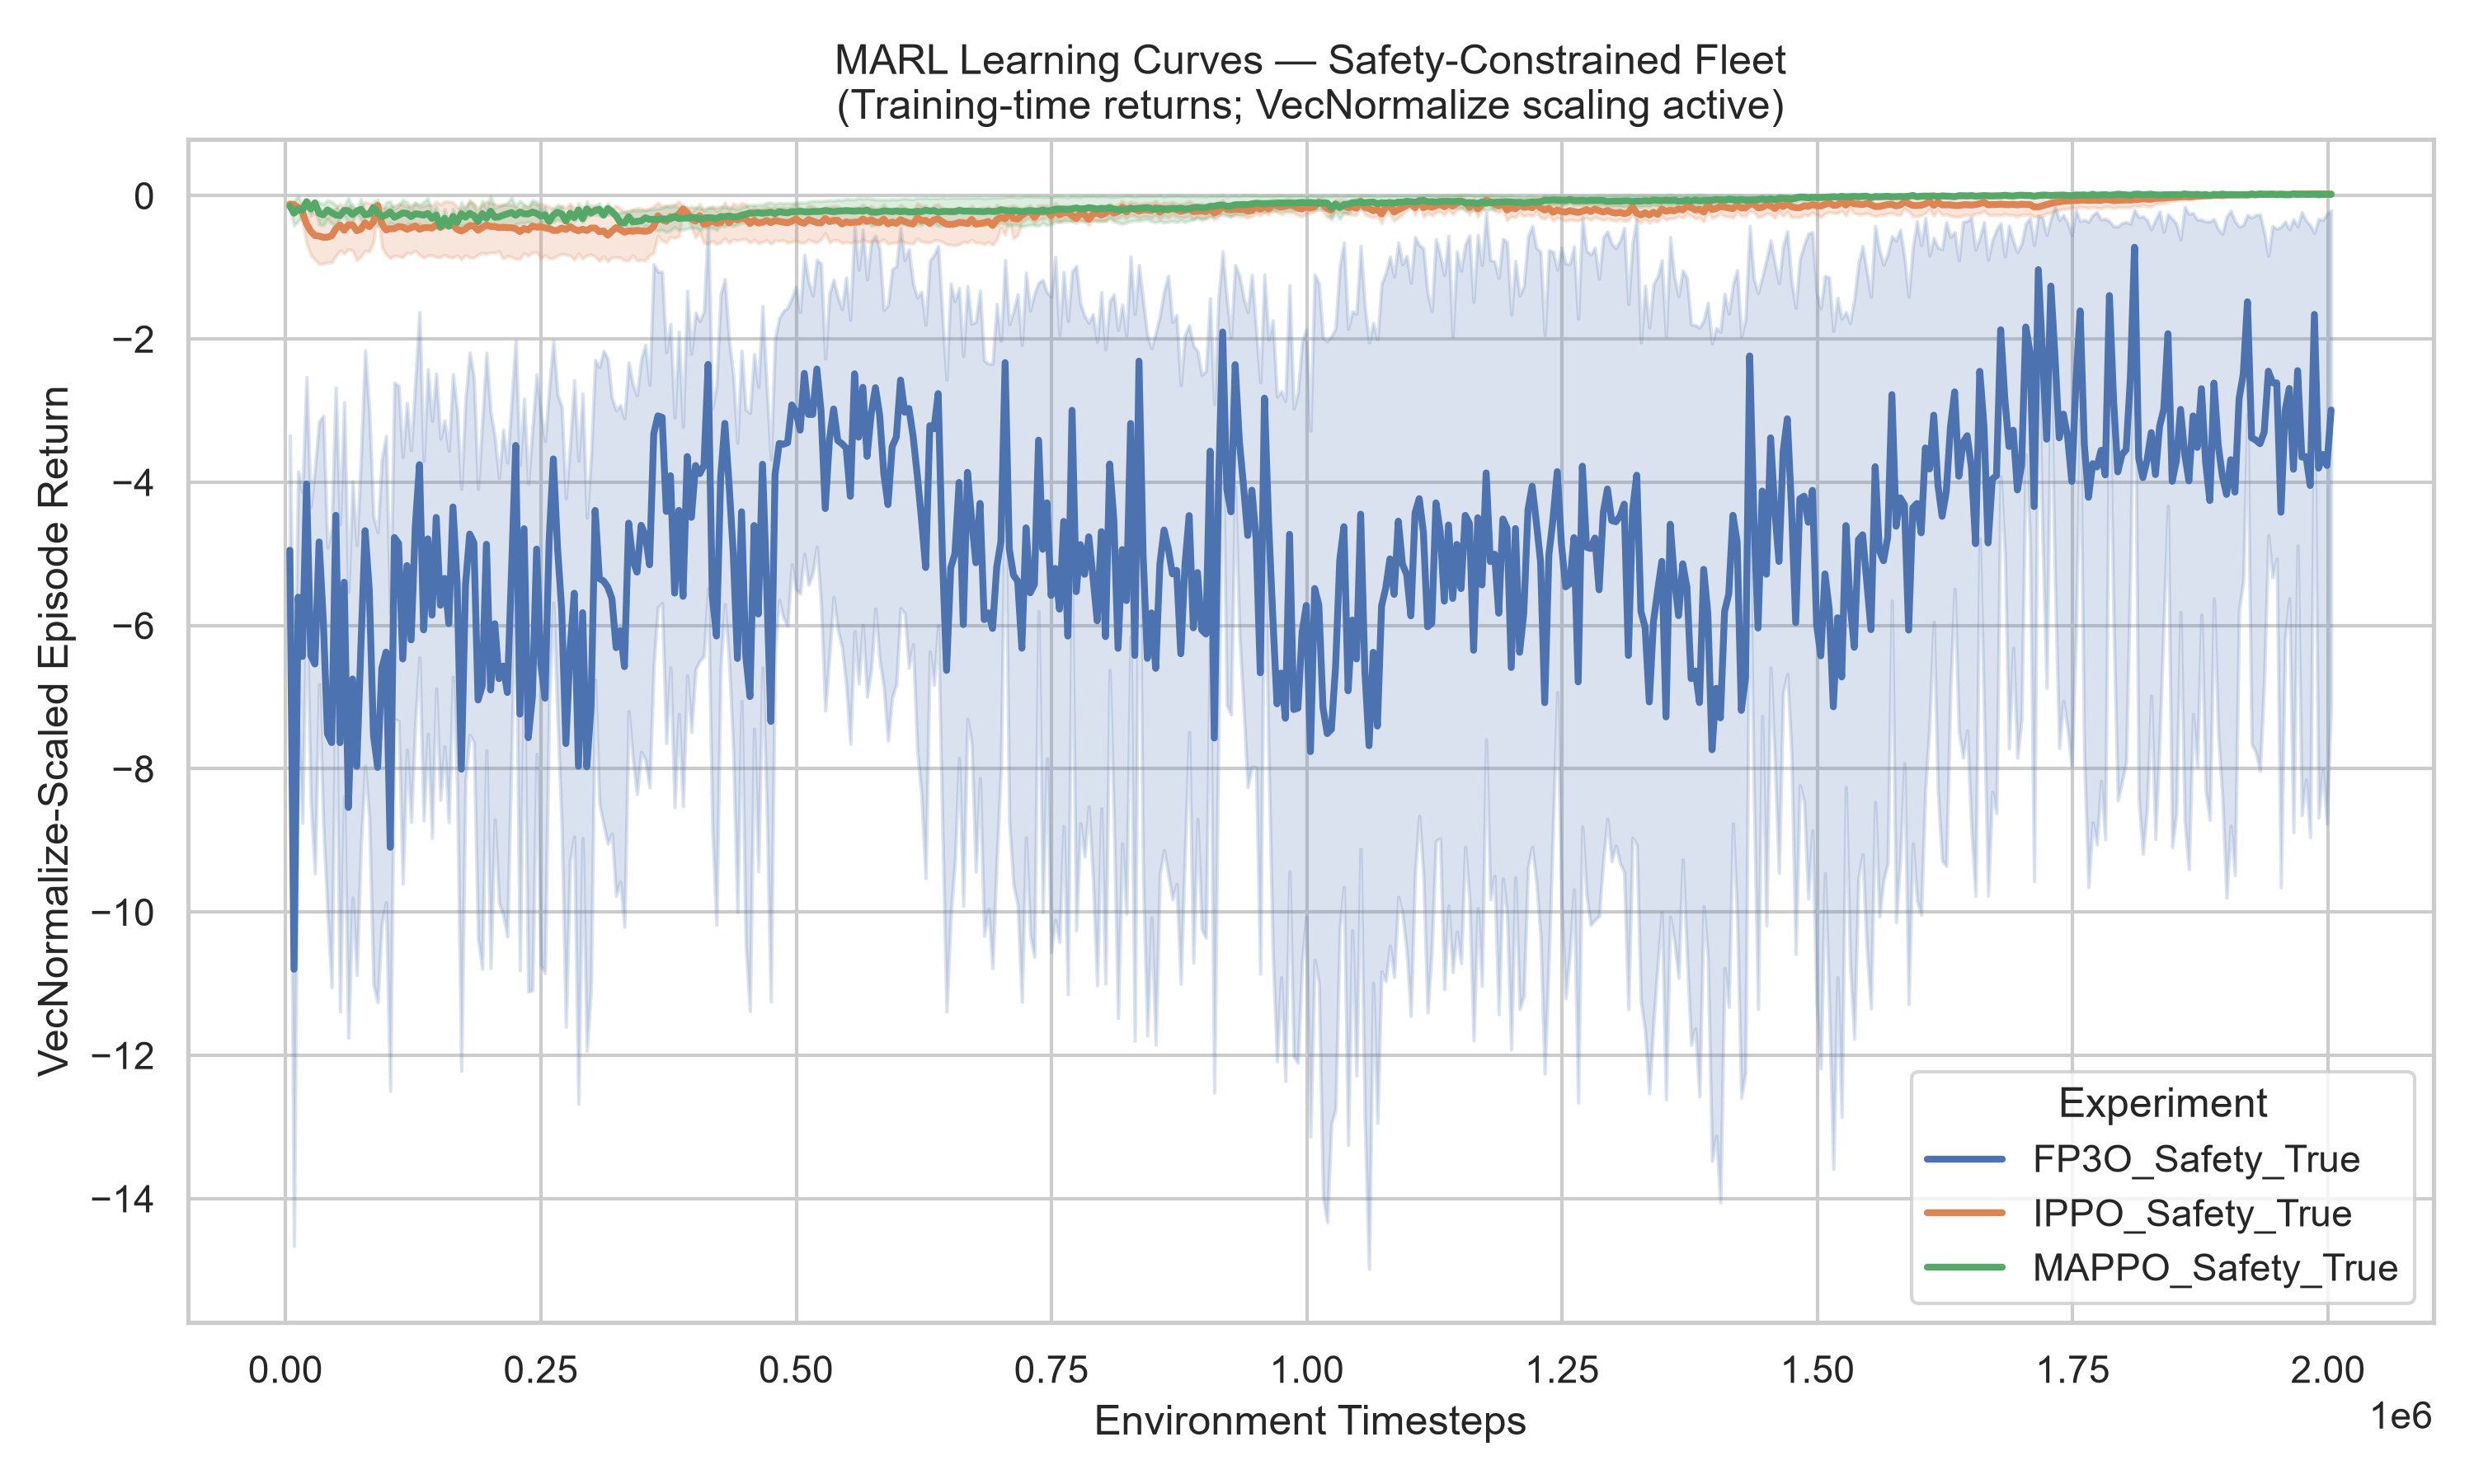
\includegraphics[width=0.92\textwidth]{figures/learning_curves.png}
\caption{Earlier isolated-channel training-time learning curves across the retained safety-constrained runs. The FP3O trace exhibits much larger return variance than the shared-policy baselines. This figure is historical diagnostic evidence and is not the primary coupled-channel benchmark.}
\label{fig:learning}
\end{figure}

\begin{figure}[H]
\centering
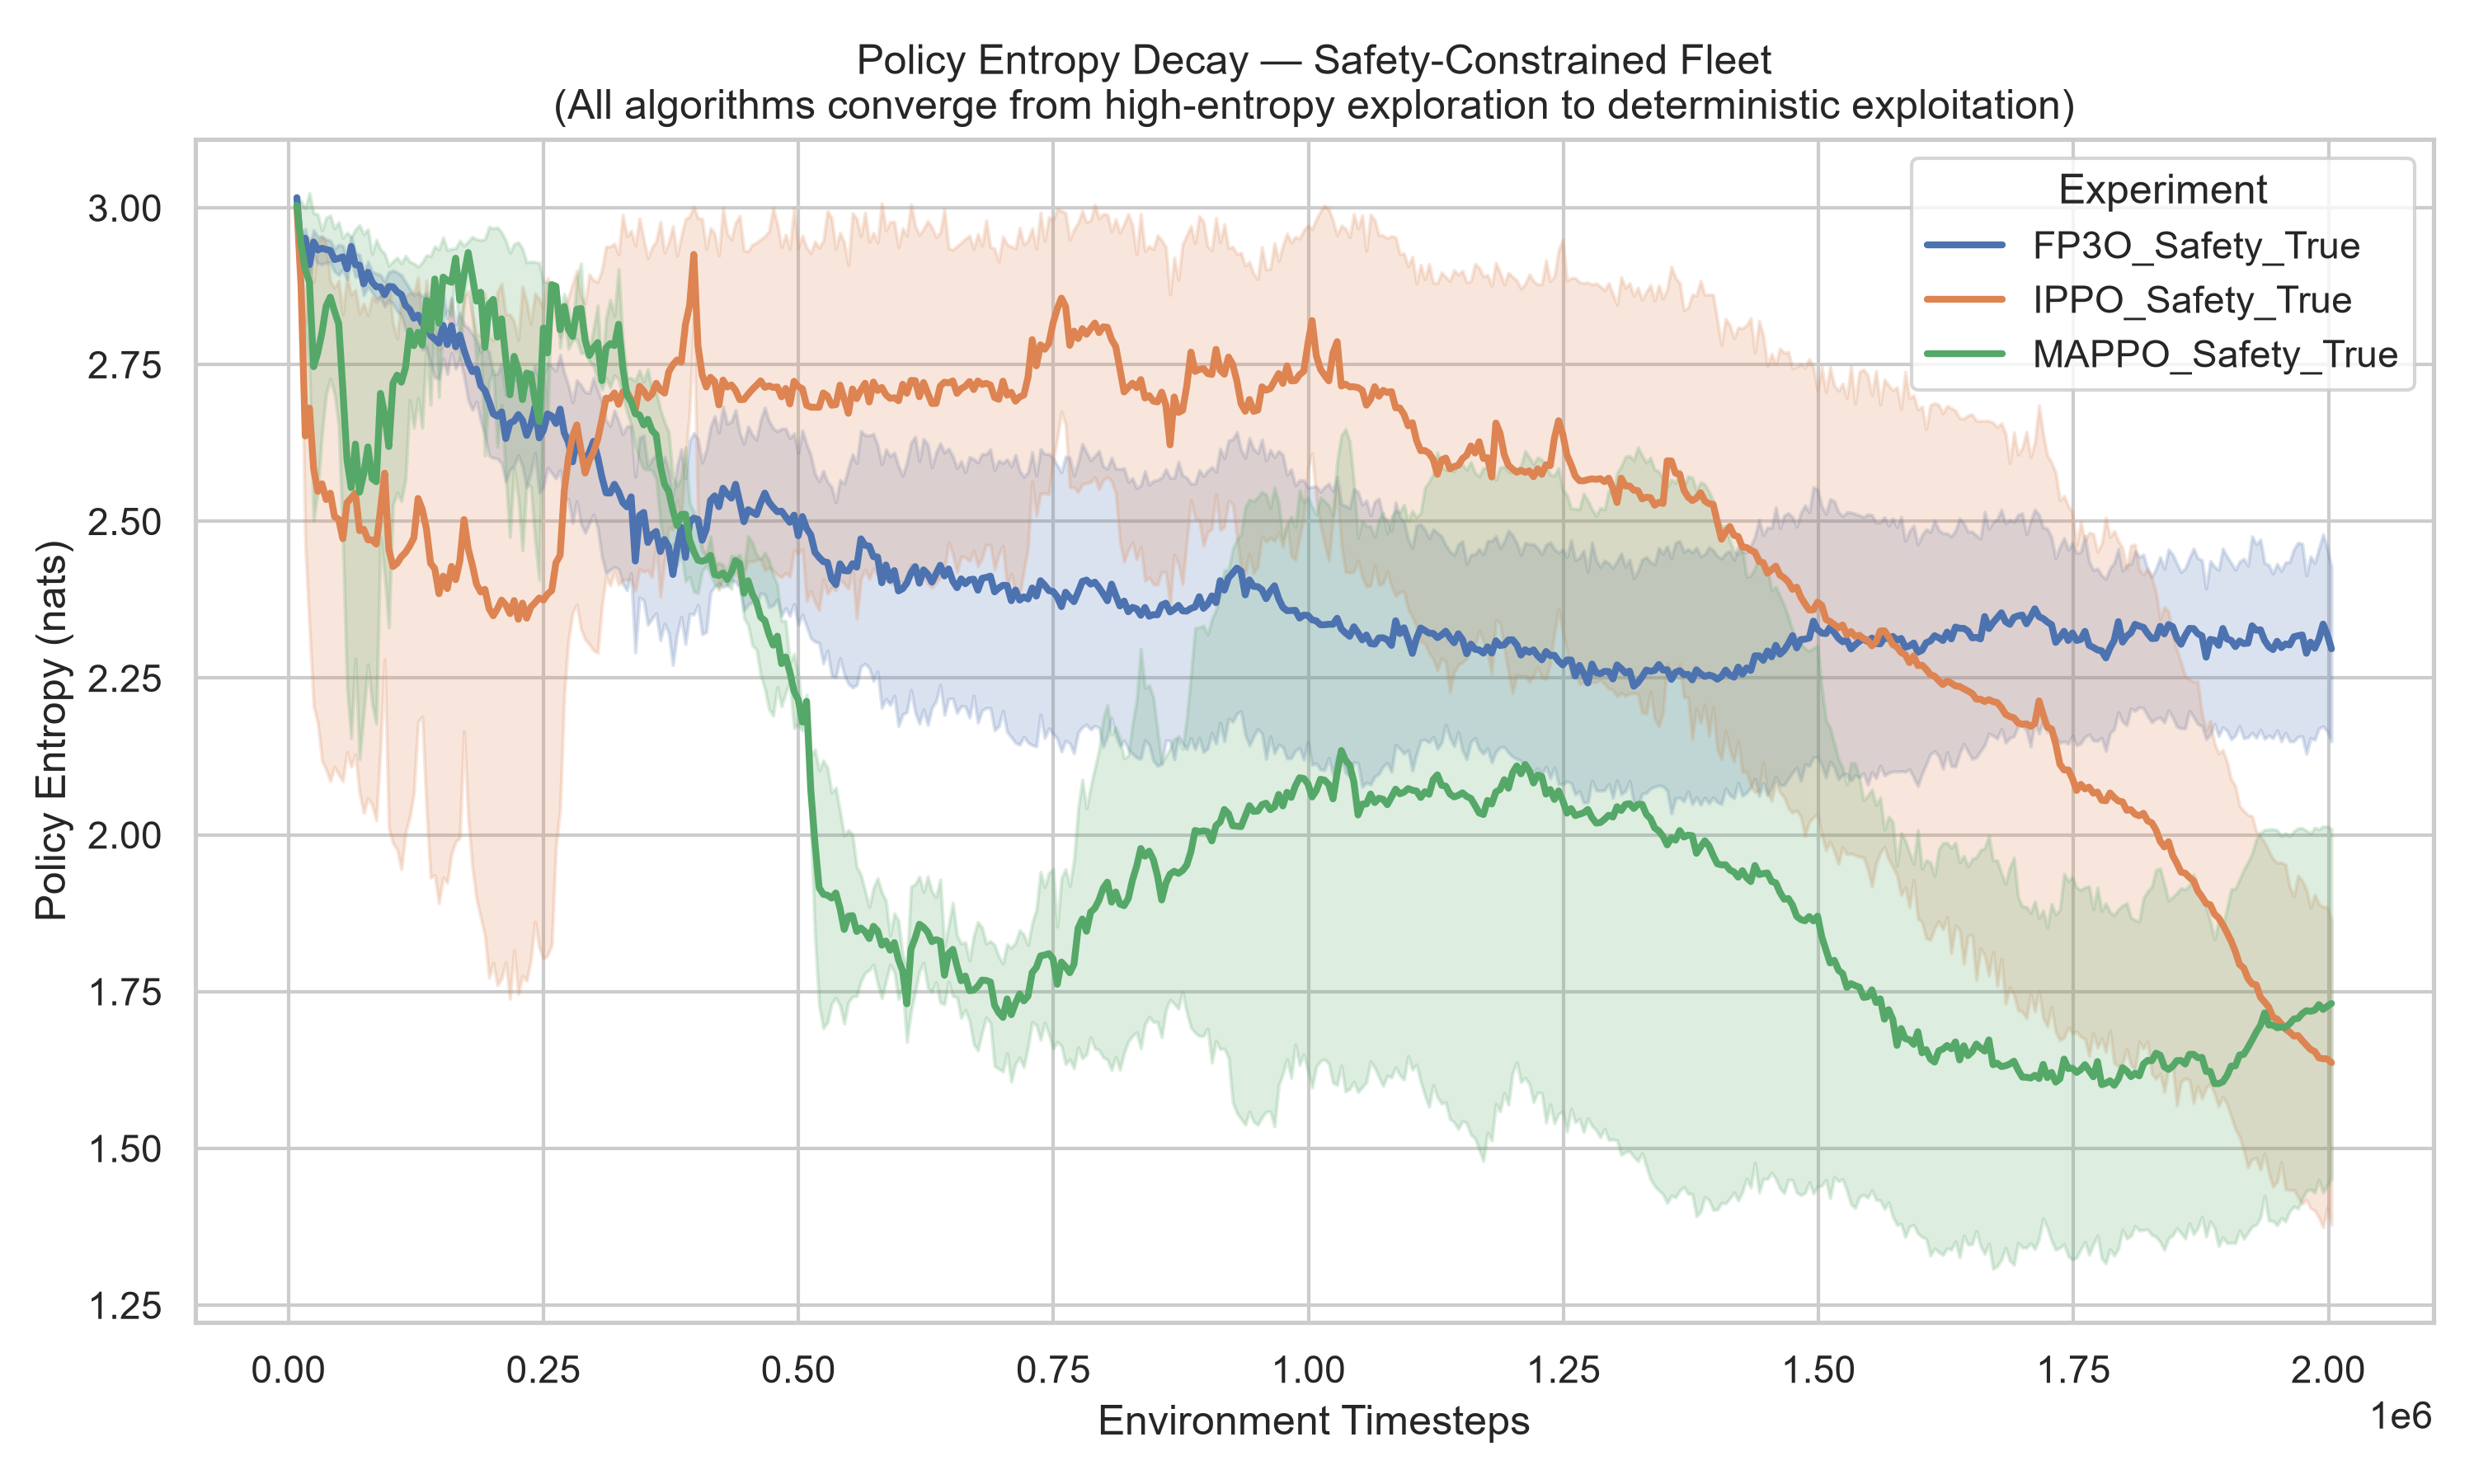
\includegraphics[width=0.92\textwidth]{figures/entropy_curves.png}
\caption{Earlier isolated-channel policy-entropy diagnostics. The figure is retained to document the development-stage observation that FP3O's training dynamics were more variable than those of the shared-policy baselines.}
\label{fig:entropy}
\end{figure}

\begin{figure}[H]
\centering
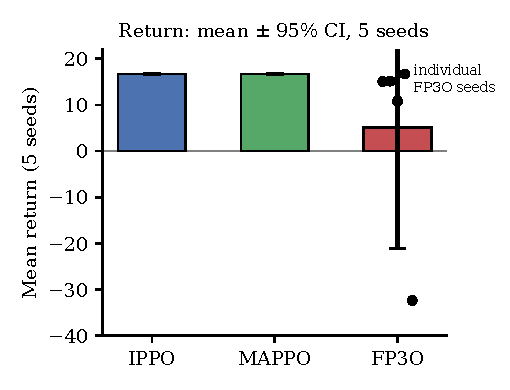
\includegraphics[width=0.62\textwidth]{figures/algo_comparison_3way.pdf}
\caption{Earlier five-seed isolated-channel comparison of type-conditioned IPPO, MAPPO, and FP3O. The FP3O distribution is dominated by one low-return seed. This historical comparison motivated the later introduction of coupled-channel contention and should not be confused with the updated six-configuration benchmark.}
\label{fig:isolatedcomparison}
\end{figure}

\section{Statistical Interpretation}
The updated paper reports that IPPO Blind and FP3O Type-conditioned are statistically indistinguishable at the available sample size. The thesis therefore emphasizes effect direction and engineering diagnostics rather than overclaiming significance. Five seeds are useful for exposing seed-level instability, but they are still a small sample for estimating the tail behavior of a stochastic training process.

The central evidence can be summarized as follows:
\begin{itemize}[leftmargin=*]
    \item Type-conditioned shared policies are highly competitive in isolated settings.
    \item Coupled contention changes the behavior of the comparison: type conditioning harms the two shared-actor baselines in the 100k regime.
    \item FP3O benefits strongly from receiving the same semantic type information because the type vector can route observations to its specialized heads.
    \item FP3O Type-conditioned has the lowest shield intervention rate in the primary benchmark.
    \item All six configurations eventually approach the same reward ceiling in long-horizon runs, so the 100k result is primarily an early-training and safety-behavior result.
\end{itemize}

\chapter{Discussion and Limitations}

\section{What the Results Mean}
The research began with a binary architectural question: is specialization necessary? The staged experiments show that this binary formulation is too coarse. This interpretation is consistent with prior work showing that parameter sharing can be highly effective in cooperative MARL, while its behavior depends on how agent-specific information is represented \parencite{yu2022surprising,terry2020revisiting}.

In the isolated environment, shared semantic conditioning is sufficient to produce very strong policies. This finding is important because it prevents an overly simple conclusion that every heterogeneous MARL problem requires separate heads. Parameter sharing remains an efficient and competitive default when the agents are heterogeneous in role but not strongly coupled through a shared physical bottleneck.

The coupled-channel experiment adds a different pressure. Multiple agents now influence the same effective bandwidth, so their actions have an externality beyond their own ECU. This is precisely the type of interaction that motivates centralized critics and explicit cooperative coordination mechanisms in MARL \parencite{lowe2017maddpg,foerster2018coma,yu2022surprising}. The architecture must represent both role-specific operation preferences and temporal coordination. In this setting, explicit FP3O heads become useful because the semantic type signal can route the shared representation into distinct final policy distributions.

The evidence is strongest when stated conditionally: \emph{explicit specialization becomes more valuable as heterogeneous roles are coupled through a shared communication resource, at least during the early training regime studied here}. The long-horizon result prevents this statement from being interpreted as an asymptotic performance theorem.


\section{Engineering Interpretation of the Coupled Result}
The coupled-channel experiment changes the meaning of a locally attractive action. In an isolated channel, an ECU can evaluate the relative cost of its own update operation largely through its own state and role preference. Under the shared gateway, the same action also changes the effective communication condition faced by other transmitting agents. The learning problem therefore contains an externality: an action that appears inexpensive for one ECU can increase contention for the team. This is the principal reason the coupled benchmark is treated as the authoritative setting for the specialization question.

The result does not imply that one architecture is universally preferable. Prior comparative studies likewise show that PPO-based MARL performance is sensitive to environment structure and implementation details, which supports treating the present result as a controlled case study rather than a universal ranking \parencite{yu2022surprising,feng2023fp3o,zhong2023harl}. The primary benchmark contains two different dimensions of performance. On return, IPPO without type conditioning has the highest sample mean, while the uncertainty is sufficiently large that the reported comparison with FP3O type conditioning is not statistically decisive at the available number of seeds. On safety behavior, FP3O type conditioning has the lowest intervention rate. These observations support a conditional engineering interpretation. If the only objective is the reported early-training return, the evidence does not justify declaring FP3O the winner. If reducing reliance on the external safety filter is also a first-class objective, the specialized type-conditioned configuration becomes more attractive.

The long-horizon validation further narrows the scope of the claim. Since all six configurations approach a similar empirical ceiling, the strongest difference appears to concern the path by which policies learn rather than the maximum return that can eventually be reached in the present simulator. This matters for deployment-oriented research because training budget and online adaptation cost can be important, but it also prevents the thesis from converting a transient advantage into a universal asymptotic statement.

\section{Implications for OTA Scheduling Research}
The results suggest that representation design should be treated as part of the system model rather than as a purely neural-network implementation choice. In a heterogeneous scheduling problem, the meaning of an observation determines what distinctions a shared policy can represent. Semantic role information can provide the network with the information needed to select different operations without requiring a separate network for every agent. At the same time, a shared bottleneck can make the coordination problem richer than independent role-conditioned decision making.

For future OTA schedulers, this suggests a practical workflow. The first model should establish whether a shared policy with explicit semantic conditioning can solve the task efficiently. This recommendation is aligned with prior findings that parameter sharing can provide strong sample efficiency while agent indications and heterogeneous roles affect what a shared policy can represent \parencite{terry2020revisiting,terry2021pettingzoo}. Specialization should then be introduced when there is evidence of systematic role conflict, cross-agent coupling, or persistent safety dependence that a shared representation does not handle well. Such a progression avoids assuming that either full sharing or full separation is inherently superior. It also aligns the architecture decision with measurable properties of the environment.

\section{Limitations of the Experimental Abstraction}
The controlled environment necessarily omits several sources of complexity present in operational OTA systems. It does not model cryptographic verification cost, complete diagnostic state machines, detailed retransmission behavior, ECU reboot dependencies, real firmware dependency graphs, or heterogeneous compute resources. The channel model is stochastic but intentionally compact, and the gateway coupling is a bandwidth-sharing abstraction rather than a full network scheduler. These omissions do not invalidate the controlled comparison, but they limit the domain to which the numerical values can be transferred.

The synthetic ECU multipliers are another limitation. They create a reproducible form of behavioral conflict, but a measured production fleet could exhibit different cost relationships. A future study should therefore preserve the experimental methodology while replacing synthetic multipliers with calibrated traces or publicly documented update characteristics. Likewise, larger fleets may change the computational cost of exact Shapley calculations and the nature of representation sharing. The present four-agent result should consequently be treated as a validated case study, not a scaling guarantee.

\section{Why Type Conditioning Is Not Equivalent to Agent Identity}
The confound correction is one of the methodological contributions of the thesis. Suppose the policy receives an identity vector $e_i$ and the environment permanently maps each identity to a different ECU role. Then
\begin{equation}
P(\text{type}\mid\text{agent ID})=1,
\end{equation}
so the policy can infer type from identity. But the identity also distinguishes agents within the same role. The policy can therefore implement $\pi_i(a\mid o)$ for each physical agent while using one network.

With semantic type conditioning, the desired property is instead
\begin{equation}
\pi(a\mid o,\text{type}=k),
\end{equation}
so two agents of the same type share the same conditioning signal. This makes the policy represent role-dependent behavior without giving it a unique key for memorization. The distinction is directly relevant to fair comparisons of parameter sharing \parencite{terry2020revisiting}.

\section{Representation Interference as a Behavioral Pattern}
The updated paper uses the term Representation Interference because the shared baselines deteriorate after semantic type conditioning while FP3O improves. The term should not be confused with a direct gradient-conflict measurement. A true gradient-level claim would require logging the per-type gradient vectors and measuring quantities such as pairwise cosine similarity or conflicting update components.

The current evidence is therefore best interpreted as an empirical interaction effect between architecture and conditioning under gateway contention. This interpretation is narrower than claiming a universal mechanism, and it is consistent with prior work showing that heterogeneous-agent representation and parameter-sharing choices can materially affect cooperative learning behavior \parencite{terry2020revisiting,zhong2023harl,feng2023fp3o}. Future work should explicitly measure per-type gradient similarity and compare it with the return and shield-rate changes reported here.

\section{Safety as a Second Evaluation Axis}
In a safety-relevant application, optimizing return alone can be misleading. A policy may appear successful because an external governor repeatedly prevents dangerous actions. The shield-rate metric exposes this dependence.

FP3O Type-conditioned has the lowest shield rate in the primary benchmark, while IPPO Blind has the highest raw return. This produces a genuine engineering trade-off: if a system designer values low intervention as evidence that the learned policy itself has internalized the constraint, FP3O Type-conditioned is attractive even though it is not the highest-return row.

The thesis does not equate lower shield use with formal safety certification. The shield itself remains the mechanism that enforces the hard memory condition.

\section{Limitations}
\begin{itemize}[leftmargin=*]
    \item \textbf{Synthetic firmware and channel traces.} Firmware blocks, similarity values, and stochastic channel parameters are generated by the simulator. No proprietary production firmware or vehicle telemetry is used.
    \item \textbf{Small fleet size.} The headline experiments use four agents. Larger fleets could produce different contention patterns and may make Shapley estimation more difficult.
    \item \textbf{Small seed count.} Five seeds expose important variability but are insufficient for strong claims about rare training failures.
    \item \textbf{Undiagnosed FP3O failure mode.} The project observed a severe low-return FP3O seed in the earlier isolated benchmark. The exact cause, whether numerical instability, masking interaction, optimization dynamics, or a bad local solution, has not been conclusively isolated.
    \item \textbf{Modelled gateway physics.} The bandwidth-sharing rule is deliberately simple. Real cellular scheduling, packet retransmission, protocol overhead, and radio resource allocation are more complicated.
    \item \textbf{Safety-shield abstraction.} The filter is CBF-inspired but not a formal CBF certificate for a production ECU network.
    \item \textbf{Payload target gap.} The learned payload costs remain above the project's 5,000-byte engineering target, so deployment readiness is not established.
    \item \textbf{Configuration lineage.} The public repository contains legacy scripts and historical configuration names alongside the newer coupled-channel runner. Reproducibility therefore requires using the main experiment runner and recording all relevant CLI flags rather than relying on every legacy default.
\end{itemize}

\section{Threats to Validity}
Internal validity is strongest where the six coupled-channel configurations share the same environment, seed count, training horizon, and evaluation procedure. The repository's automated environment and policy tests provide an internal reproducibility check for the implementation used in these comparisons \parencite{ma_reles_ota_repo}. The principal internal threat is the possibility that a remaining implementation detail interacts differently with each architecture. The repository's automated environment and policy tests reduce this risk but do not eliminate it.

Construct validity is limited by the simplified cost model. Operation multipliers represent controlled role preferences rather than measured production ECU costs. Similarly, shield intervention rate is a useful behavioral proxy for safety reliance, not a formal safety metric.

External validity is limited because the simulator does not model a complete automotive communication stack or production-grade OTA security workflow. Real automotive OTA systems involve security, diagnostic, connectivity, and deployment considerations that extend beyond the controlled scheduling abstraction used here \parencite{halder2020survey,ghosal2022stride,shoker2023scalota}. The results should therefore be read as evidence about a controlled MARL scheduling problem motivated by automotive OTA systems, not as a direct benchmark of a commercial vehicle platform.

\section{Reproducibility}
The repository provides the environment, shared OTA physics, policy implementation, experiment runner, evaluation utilities, tests, and experiment logs \parencite{ma_reles_ota_repo}. The thesis preserves both the current primary figures and selected historical figures so that the progression from isolated to coupled experiments is visible. All headline results are reported at seed level rather than being reconstructed from a single aggregate run.

\chapter{Conclusion}

\section{Summary of the Research}
This thesis extended a single-agent OTA scheduling problem into a heterogeneous cooperative MARL environment and used it to study the boundary between parameter sharing and explicit specialization. The work combined four important components: shared OTA physics, heterogeneous ECU operation preferences, a safety shield, and Shapley-valued credit assignment.

The experimental design evolved in response to evidence. Homogeneous and uniformly heterogeneous settings showed that specialization provides little benefit when there is little qualitative behavioral conflict. A later experiment exposed a methodological confound caused by a raw agent identifier. Replacing that identifier with semantic ECU type produced a fairer comparison and demonstrated that shared policies can remain extremely competitive in isolated settings.

The updated research then introduced the key physical coupling: a shared gateway whose bandwidth is divided among concurrent transmitting agents. The five-seed, 100,353-step benchmark revealed a strong architecture-by-conditioning interaction. Type conditioning lowered the mean return of IPPO and MAPPO but raised FP3O by 111.44 points. FP3O Type-conditioned also had the lowest safety-shield intervention rate. However, its return was not statistically distinguishable from the best shared baseline at the available sample size, and all six configurations eventually approached the same reward ceiling in the 2,000,897-step validation.

\section{Answers to the Research Questions}
\textbf{RQ1: Can the ReLES-OTA formulation be extended to MARL?} Yes. The resulting PettingZoo environment supports concurrent ECU agents, variable-length completion, action masks, heterogeneous costs, stochastic channel conditions, and a fleet-level safety mechanism.

\textbf{RQ2: Is semantic type conditioning sufficient in isolated settings?} The project evidence indicates yes for the studied four-agent isolated environment. Type-conditioned IPPO and MAPPO reached the same strong long-horizon return, while FP3O introduced additional seed instability without a demonstrated significant return advantage.

\textbf{RQ3: Does specialization become more useful under coupled contention?} The 100k benchmark provides qualified evidence in that direction. FP3O benefits dramatically from type conditioning while the shared baselines degrade. The effect is behavioral and early-training; it is not an asymptotic theorem.

\textbf{RQ4: Does safety behavior change the preferred architecture?} Yes. FP3O Type-conditioned has substantially lower shield intervention than IPPO Blind in the primary benchmark. Therefore, the preferred operating point depends on whether the system is evaluated solely by return or jointly by return and learned-policy reliance on the safety governor.

\section{Main Contributions}
The thesis contributes a reproducible MARL formulation for OTA scheduling, a controlled heterogeneous cost model, an explicit shared-gateway coupling mechanism, a methodology for avoiding identity leakage in parameter-sharing experiments, and a safety-aware evaluation framework. More broadly, it demonstrates why architecture comparisons in heterogeneous MARL should report observation semantics, coupling assumptions, seed distributions, and safety interventions rather than only a single mean return.

\section{Future Work}
Future work should first expand the number of independent seeds and report effect sizes and confidence intervals with greater statistical power. Second, the FP3O low-return seed should be instrumented at the gradient and head level to determine whether its failure is numerical, architectural, or data-distribution driven. Third, the coupled gateway should be replaced or augmented with a richer wireless model containing scheduling, retransmission, and protocol overhead. Fourth, the synthetic firmware model should be calibrated with anonymized or public OTA traces where possible. Finally, experiments should scale beyond four ECUs and sixteen blocks and should test whether the conditional specialization benefit persists when fleets contain multiple agents of the same type.

\section{Final Remarks}
The strongest conclusion of this work is not that FP3O always beats IPPO or MAPPO, nor that parameter sharing is always sufficient. The evidence instead points to a more useful design principle: \emph{the value of policy specialization depends on how role heterogeneity interacts with physical coupling}. In an isolated environment, semantic conditioning can provide most of the benefit of specialization while preserving the simplicity of a shared policy. Under a shared communication bottleneck, explicit role-specific heads can substantially improve early coordination and reduce reliance on an external safety filter. Establishing whether this advantage persists with larger fleets, richer channel physics, and stronger statistical power is the next step toward a deployment-relevant conclusion.

%-------------------------- BACK MATTER --------------------------%
\printbib

\begin{appendices}

\chapter{Reproducibility Configuration}

The following table summarizes the parameters associated with the reported research. The primary coupled-channel benchmark follows the provided research manuscript; the public repository contains additional legacy defaults and command-line options, so all reproduction attempts should record the full experiment command and configuration.

\begin{table}[H]
\centering
\small
\begin{tabular}{ll}
\toprule
Parameter & Primary value\\
\midrule
ECU agents & 4\\
Firmware blocks per agent & 16\\
ECU types & Engine, braking, infotainment, generic\\
Gateway bandwidth & 25 Mbps\\
Safety threshold & 85\% of memory budget\\
Primary horizon & 100,353 steps/seed\\
Long horizon & 2,000,897 steps/seed\\
Seeds per configuration & 5\\
Parallel environments & 4\\
Rollout horizon & 256\\
Mini-batch size & 128\\
PPO epochs & 10\\
Learning rate & $3\times10^{-4}$\\
Discount factor & 0.99\\
GAE $\lambda$ & 0.95\\
Clip range & 0.2\\
\bottomrule
\end{tabular}
\caption{Primary experimental configuration synthesized from the updated research manuscript and the maintained repository.}
\label{tab:repro}
\end{table}

\section{Repository Reconciliation Notes}
The maintained repository is the implementation source for the environment and experiment pipeline \parencite{ma_reles_ota_repo}. A few legacy defaults differ from the final benchmark settings used by the updated paper. In particular, the configuration module currently centralizes a four-environment rollout, 256-step horizon, batch size 128, entropy coefficient 0.001, and target KL 0.05, while some older function signatures and legacy scripts still expose different defaults. The thesis therefore avoids presenting those legacy defaults as experimental evidence.

The current repository's shared OTA physics uses a truncated Gaussian latency with mean 120 ms, standard deviation 40 ms, and bounds 50--200 ms. This is the implementation-level parameterization. The updated paper should remain the authoritative source for the exact configuration associated with its reported numerical results.


\chapter{Detailed Reproduction and Reporting Checklist}
This appendix provides a structured checklist for reproducing the experiments and for interpreting future extensions without changing the scientific meaning of the comparison.

\section{Environment Consistency}
A reproduction should verify that the number of agents, firmware blocks, ECU-type mapping, action encoding, action masks, reward coefficients, safety threshold, and channel configuration match the intended benchmark. These parameters jointly define the decision problem. Changing several of them while preserving the same algorithm name does not reproduce the reported experiment. In particular, isolated and coupled channels should never be treated as interchangeable because the coupled environment introduces a direct cross-agent externality.

The shared OTA cost engine should also remain common across algorithmic conditions. A convenient optimization in one training script can otherwise create an accidental implementation advantage. The repository structure is useful here because the environment, training pipeline, evaluation utilities, and result-generation tools are maintained as explicit artifacts rather than as undocumented notebook state \parencite{ma_reles_ota_repo}. Reproduction should record the repository revision used for a run in addition to the numerical hyperparameters.

\section{Observation Audit}
Before training, every observation component should be classified as local, global, semantic, or identity-specific. Local information describes the agent's own backlog or resource state. Global information is available only where the CTDE design permits it, such as to a centralized critic. Semantic information describes a meaningful role, for example ECU type. Identity-specific information identifies an individual agent.

This audit is important because identity can leak semantics. If every run assigns the engine role to the same index, an identifier can function as a role label. A shared network can then learn a different response for each index, which changes the effective hypothesis being tested. When the goal is to test semantic conditioning, the type vector should carry the intended role information and any raw identifier should be removed unless identity itself is a deliberate experimental variable \parencite{terry2020revisiting}.

\section{Training and Seed Protocol}
Each seed should start from a fresh initialization. Model checkpoints from one seed must not be silently reused as initialization for another seed because this would invalidate the interpretation of independent repetitions. The exact number of timesteps should be recorded per seed, together with the number of parallel environments, rollout horizon, batch size, PPO epochs, learning rate, discount factor, GAE parameter, clip range, entropy coefficient, and any KL-based stopping rule. These settings affect optimization dynamics and can change early-training comparisons substantially \parencite{raffin2021sb3}.

When extending the study, additional seeds are preferable to repeating narrative claims based on one exceptional trajectory. Seed-level results should be retained so that alternative uncertainty estimates and effect sizes can be calculated later. If an experiment is stopped early, the reason should be logged because early termination can otherwise bias a comparison toward configurations that happened to improve faster.

\section{Evaluation Separation}
Training metrics and evaluation metrics should be kept distinct. A training return can be influenced by exploration and by the evolving policy during data collection. A deterministic evaluation on fresh episodes answers a different question: how the trained policy behaves under a fixed evaluation procedure. Both can be useful, but they should not be merged without labeling. The maintained software artifact includes evaluation utilities, allowing future work to make this separation explicit \parencite{ma_reles_ota_repo}.

For safety-aware evaluation, both proposed and executed actions are conceptually important. If the shield changes an action, the executed transition may look safe even though the policy itself proposed an unsafe alternative. Reporting intervention rate therefore provides information that a final return cannot reveal. Future versions may additionally log the severity and type of proposed violations, provided those quantities are defined consistently across architectures.

\section{Result Interpretation Checklist}
Before stating an architectural conclusion, the following questions should be answered:
\begin{enumerate}[leftmargin=*]
    \item Are all compared conditions solving the same environment instance and using the same training budget?
    \item Does each architecture receive comparable semantic information at execution time?
    \item Could any observation feature allow hidden memorization of agent identity?
    \item Are the reported means accompanied by seed variability or confidence intervals?
    \item Is a statistically non-significant comparison being described conservatively rather than as proof of equality?
    \item Are early-training and long-horizon findings clearly separated?
    \item Does a safety conclusion refer to shield behavior in the simulator rather than formal real-world certification?
    \item Does any proposed internal mechanism have direct measurements supporting it?
\end{enumerate}

Applying these checks helps preserve the central contribution of the thesis: the comparison is not only about which algorithm obtains a better number, but about whether the information, coupling, and evaluation design justify the architectural interpretation attached to that number.

\chapter{Monte Carlo Shapley Credit Assignment}

For $N$ agents, let $v(S)$ be the coalition value obtained when only agents in $S$ participate. The Shapley value of agent $i$ is
\begin{equation}
\phi_i(v)=\frac{1}{N!}\sum_{\pi\in\Pi}\left[v(P_i^\pi\cup\{i\})-v(P_i^\pi)\right],
\end{equation}
where $\Pi$ is the set of all permutations of the agents and $P_i^\pi$ is the set of agents preceding $i$ in permutation $\pi$ \parencite{shapley1953value}.

For four agents, $4!=24$ permutations are small enough to enumerate exactly. The implementation evaluates coalition contributions for these permutations and assigns each agent the resulting marginal contribution, with the progress term added separately. For larger fleets, sampling a subset of permutations becomes attractive because the factorial enumeration grows rapidly \parencite{castro2009shapley}.


\chapter{Extended Methodological Rationale}
\section{Why the Study Uses a Staged Design}
The final coupled-channel benchmark is the endpoint of a sequence of increasingly demanding environments. This progression is methodologically useful because a single final experiment cannot explain why an architecture succeeds or fails. A homogeneous setting first tests whether the implementation can learn a common scheduling problem. Uniform heterogeneity then checks whether superficial differences in agents are sufficient to create a specialization advantage. Structural heterogeneity introduces deliberately conflicting operation preferences, making role-sensitive behavior meaningful. The identity-confound stage verifies that the observation design does not accidentally answer the specialization question before learning begins. The isolated semantic-conditioning stage then measures the representational capacity of a shared policy when it receives legitimate role information. Finally, the coupled channel adds a resource interaction that requires coordination beyond purely local operation choice.

Each stage therefore eliminates a different alternative explanation. If specialization helped only after structural heterogeneity, the likely explanation would involve role conflict rather than an implementation artifact. If a shared policy became strong after semantic conditioning, this would show that one network can represent multiple role-dependent behaviors without separate parameters. If a difference reappeared after gateway coupling, the interpretation would shift toward coordination under interaction. This staged logic is more informative than treating every historical experiment as an independent leaderboard.

\section{Why PPO-Based Comparators Are Used}
The purpose of the thesis is to study how representation sharing interacts with heterogeneous roles, not to establish a universal ranking of all MARL families. PPO provides a common optimization framework within which independent and centralized-training variants can be compared. MAPPO and related implementations have demonstrated that carefully designed PPO-based baselines can be highly competitive in cooperative MARL tasks \parencite{yu2022surprising}. Keeping the optimization family similar also reduces the number of confounding differences when interpreting architecture changes.

IPPO serves as a decentralized baseline in which agents optimize from their own actor-side information. MAPPO introduces centralized value information during training while preserving decentralized execution. FP3O introduces an explicit mechanism for different parameter-sharing structures within the PPO pipeline \parencite{feng2023fp3o}. The comparison should therefore be read as a structured design study: how much coordination and specialization are useful for this OTA environment under comparable training procedures.

\section{Role of Centralized Training}
Centralized training does not mean centralized deployment. During training, additional information can be used to construct a critic or training signal, while each actor remains restricted to its intended execution-time observation. This separation is particularly relevant to vehicular OTA scheduling because a centralized fleet manager may have broad state visibility during planning or offline training, whereas deployed controllers may need to make decisions using local and semantically available information.

The thesis does not claim that every vehicle architecture can support the same information pattern. Instead, CTDE provides a controlled way to examine whether richer training-time information improves learning without requiring the final actor to depend on the full fleet state. This design follows the broader centralized-critic literature while preserving the decentralized execution question central to MARL \parencite{lowe2017maddpg,foerster2018coma}.

\section{Why Action Masking Is Part of the Environment}
Invalid actions are not treated as ordinary bad choices with a large negative reward. A firmware block that has already been completed is unavailable, so sampling it as though it were a legitimate action would enlarge the learning problem with meaningless alternatives. The environment therefore exposes a mask that removes invalid block selections before action sampling. This keeps the policy focused on feasible decisions while preserving the changing action availability that naturally arises as blocks are completed \parencite{huang2022masking}.

Masking must remain consistent across all architectures. If one policy receives an exact feasibility mask while another learns feasibility only through penalties, the experiment compares both representation and constraint handling. The present design instead keeps action feasibility as a common environment interface so that differences are interpreted primarily through sharing, conditioning, and centralized training.

\section{Why Exact Shapley Enumeration Is Feasible Here}
Credit assignment is difficult when the reward is generated by a joint outcome. The Shapley value provides a principled allocation based on average marginal contribution across coalitions \parencite{shapley1953value}. Its direct calculation is expensive for large teams because the number of permutations grows factorially. For the four-agent setting, however, only 24 permutations exist. Exact enumeration is therefore computationally manageable and avoids sampling variance in the coalition ordering itself.

This choice does not imply that exact Shapley calculation will remain appropriate for larger fleets. The implementation concept can be extended with sampling methods when the team size increases \parencite{castro2009shapley}. The present case benefits from the small fleet because it permits a clear methodological demonstration without introducing another Monte Carlo source into the reported benchmark.

\section{Why Safety Is Evaluated Separately From Reward}
A shield can improve the executed trajectory while hiding a weakness in the learned policy. Suppose two agents receive similar returns, but one repeatedly proposes actions that exceed the resource condition and relies on the shield to repair them. The final reward alone does not reveal this difference. Recording intervention frequency exposes how often the environment had to override or suppress the proposal.

This interpretation follows the general motivation for shielding and constrained learning, while remaining specific about the implementation. Formal shielding can be associated with verified specifications, and control barrier functions can provide mathematically defined invariance conditions in appropriate dynamical systems \parencite{alshiekh2018shielding,ames2019cbf}. The MA-ReLES-OTA shield is not presented as such a proof. It is a deterministic application-level filter. The useful scientific contribution is therefore behavioral measurement: architectures can be compared by how often they depend on the filter under the same simulated constraint.

\section{Generalization Boundaries}
The thesis studies generalization across random seeds and stochastic channel realizations within a fixed family of environments. It does not establish generalization across arbitrary vehicle manufacturers, firmware formats, network operators, or real traffic patterns. This distinction is important because the simulator contains controlled assumptions selected to isolate the research question.

Future validation should test several forms of distribution shift. One direction is to vary the number of ECUs and the ratio of agents sharing the same type. Another is to perturb operation multipliers and memory budgets. A third is to introduce channel regimes that differ from the training distribution. If an architecture remains stable under these changes, the evidence for a general design principle would become stronger. Until then, the thesis appropriately limits its claims to the studied environment.

\chapter{Selected Experimental Interpretation Rules}

For clarity, the thesis follows these rules when interpreting the results:
\begin{enumerate}[leftmargin=*]
    \item A more positive return is better, but return is not the only engineering metric.
    \item A lower shield intervention rate indicates less reliance on external action suppression; it does not replace the safety guarantee provided by the shield.
    \item The 100k coupled-channel benchmark is an early-training comparison, not an asymptotic performance claim.
    \item The term Representation Interference describes a behavioral architecture-by-conditioning pattern and is not a direct gradient measurement.
    \item Historical isolated-channel graphs are retained for scientific traceability and are not mixed numerically with the updated coupled-channel benchmark.
\end{enumerate}

\end{appendices}

\end{document}
